% -*- program: xelatex -*- %
\documentclass[language=english,noinputenc]{wiwwuwordrprt}

\usepackage{wiwwubildertabellen}
\usepackage{wiwwumathe}
%\usepackage{wiwwulistings}
\usepackage{wiwwuabkuerzungen}
\usepackage{etoolbox}
\usepackage{blindtext}
\usepackage{booktabs}
\usepackage{enumitem}
\usepackage[numbers]{natbib}
\usepackage{pdfpages}
\usepackage{nth}
\robustify\textellipsis
\usepackage{fontawesome}
% \usepackage{refcheck}


\usepackage{tikz-uml}
\usepackage{forest}
\usetikzlibrary{trees, arrows,shadows, positioning,chains,fit,shapes,calc, math, automata}
\usepackage{pgf-umlsd}

\usepackage[newfloat]{minted}
%\renewcommand\listoflistingscaption{List of source codes}
% \renewcommand\listingscaption{List.}
% \renewcommand{\cftlistingpresnum}{List.~}
% \captionsetup[listing]{labelformat=simple}

\usepackage{adjustbox}

\newcolumntype{R}[2]{%
    >{\adjustbox{angle=#1,lap=\width-(#2)}\bgroup}%
    l%
    <{\egroup}%
}
\newcommand*\rot{\multicolumn{1}{R{80}{1em}}}

\forestset{
  dir tree/.style={
    for tree={
      parent anchor=south west,
      child anchor=west,
      anchor=mid west,
      inner ysep=1pt,
      grow'=0,
      align=left,
      edge path={
        \noexpand\path [draw, \forestoption{edge}] (!u.parent anchor) ++(0.75em,0) |- (.child anchor)\forestoption{edge label};
      },
      font=\sffamily,
      if n children=0{}{
        delay={
          prepend={[,phantom, calign with current]}
        }
      },
      fit=band,
      before computing xy={
        l=1.5em
      }
    },
  }
}


\usepackage{amssymb}
\usepackage{pifont}
\newcommand{\cmark}{\ding{51}}%
\newcommand{\xmark}{\ding{55}}%
\newcommand{\ja}{\tiny{\cmark}}

\newlist{tabitemize}{itemize}{1}
\setlist[tabitemize]{label=\textbullet,nosep,after=\strut,leftmargin=*}

\newcolumntype{C}[1]{>{\centering\arraybackslash}m{#1}}
\newcolumntype{T}[1]{>{\riggedright\arraybackslash}p{#1}}

\usemintedstyle{tango}
\robustify\textellipsis
% \addtokomafont{section}{\clearpage}

\usepackage{fontspec}
\setmainfont[
  Ligatures=TeX,
  BoldFont={Crimson Text Bold},
  ItalicFont={Crimson Italic},
  BoldItalicFont={Crimson Text Bold Italic}
  ]{Crimson Text}
\setmonofont[Scale=0.9]{Source Code Pro}
\setsansfont{Lato}

\newcommand{\tabitem}{~~\llap{--}~~}

  \setThema{Prototypical Development of a \\Docker-based Workflow Management System}
  \setTyp{Masterthesis}
  \setFachgebiet{}
  \setLehrstuhl{Department of Information Systems \\Chair for Practical Computer Science}
  \setThemensteller{Prof.\ Dr.\ Herbert Kuchen}
  \setBetreuer{MScIS Vincent von Hof}
  \setAutor{Lars Greiving}
  \setStrasse{Dettenstraße 4}
  \setOrt{48147 Münster}
  \setTelefonnummer{+49-176 704 253 17}
  \setEMail{\textit{l\_grei02@uni-muenster.de}}
  \setAbgabetermin{2016-03-08}

\begin{document}
  \newlength{\customtabwidth}
  \setlength{\customtabwidth}{\textwidth}
  \addtolength{\customtabwidth}{-\tabcolsep}
  \captionsetup{justification=centering}
% \captionsetup[listing]{labelformat=simple}


  \EinfTitelseite

  %Verzeichnisse
  \pagenumbering{Roman} % Seitennummerierung durch roemische Ziffern
  \tableofcontents
  \listoffigures
  \listoftables
  \listoflistings

  % -*- root: ../../main.tex -*- %

\begin{AbkVerzeichnis}
  \acro{API}{Application Programming Interface}
  \acro{AMQP}{Advanced Message Queuing Protocol}
  \acro{cgroups}{control groups}
  \acro{CLI}{command line interface}
  \acro{CoW}{Copy-on-Write}
  \acro{GUI}{Graphical User Interface}
  \acro{ESB}{Enterprise Service Bus}
  \acro{JSON}{JavaScript Object Notation}
  \acro{LXC}{Linux Containers}
  \acro{OS}{Operating System}
  \acro{PID}{Process Identifier}
  \acro{REST}{Representational State Transfer}
  \acro{OASIS}{Organization for the Advancement of Structured Information Standards}
  \acro{MSA}{Micro-services Architecture}
  \acro{SOA}{Service-oriented Architecture}
  \acro{UI}{User Interface}
  \acro{WSDL}{Web Services Description Language}
  \acro{WFMC}{Workflow Management Coalition}
  \acro{WfMS}{Workflow Management System}
  \acro{WFM}{Workflow Management}
\end{AbkVerzeichnis}

  %% -*- root: ../../main.tex -*- %

\begin{Verzeichnis}{Symbolverzeichnis}
  \VerzEintrag{$a_0$}{Anschaffungsauszahlung in $t = 0$}
  \VerzEintrag{$C$}{Kapitalwert}
  \VerzEintrag{$dt$}{Einzahlungsüberschuss in bezug auf $t$}
  \VerzEintrag{$i$}{Kalkulationszinsfuß}
  \VerzEintrag{$n$}{Nutzungsdauer}
  \VerzEintrag{$q$}{Zinsfaktor $1 + i$}
  \VerzEintrag{$r_s$}{Abstand der Stufe s in cm vom Seitenrand}
  \VerzEintrag{$s$}{Stufenindex}
  \VerzEintrag{$t$}{Periodenindex}
\end{Verzeichnis}


  \clearpage
  % -*- root: ../../main.tex -*- %

\begin{abstract}
  \blindtext
\end{abstract}


  \pagenumbering{arabic} % Seitennummerierung durch arabische Ziffern

  \chapter{Introduction and motivation} % (fold)
    \label{cha:introduction_and_motivation}
    % -*- root: ../../main.tex -*- %

The digital revolution has brought with it a variety of new challenges for many enterprises, forcing the need for agility in an increasingly fragile market environment.
To cope with technological advance and competitive pressure through shortened time-to-market phases and reduced entry hurdles for market newcomers, enterprises need to adapt quickly to new technologies and business models.
Coupled with the need to optimize costs, these developments have furthered the emergence of services known as Platform as a Service (PaaS) and Software as a Service (SaaS)\cite[p.~606]{Buyya2009Cloud}.
These concepts offer a high degree of flexibility as they can be swiftly scaled to changing consumption patterns, while at the same time allow a sharing of resources among users of these services.
To be able run software in a heterogeneous infrastructure that features such services, various approaches have been presented which help to provide a predictable runtime environment \cite[p.~81]{Bernstein2014Containers}. One of them is the use of software containers which provide a way of packaging and executing processes that isolates the application from the underlying \ac{OS} of a computer and other processes that run on it.

The concept of software containers is no new notion: an early predecessor was the \texttt{chroot} command, which dates back to 1979, \emph{software jails} followed in 1998 \cite[p.~82]{Bernstein2014Containers}.
In the second decade of the \nth{21} century, solutions like Rocket, LXD, and Docker emerged, which aim at the introduction of standardized, re-usable software containers, usually in combination with tools for their management. Among these solutions, Docker is very popular. In the beginning of 2016, Docker's repository was the \nth{20} most ``starred'' repository on the source code management platform \emph{GitHub} -- ranking four positions behind the Linux kernel repository \cite{Github2016Repositories}. Docker comes with a set of utilities, which extend its main container-related functionality by features that help to set up, provision, and manage a distributed environment.

Organizations perform temporal and logical sequences of actions that help to interact with business relevant entities -- business processes -- with the objective to reach their business goals. If these processes are coordinated in an automated way, they are also called \emph{workflows}. \acp{WfMS} are designed to support the definition, execution and monitoring of these workflows \cite{Becker1999Identifying,Hollingsworth1995Wfmc}.
With regards to the challenges that heterogeneous and distributed \ac{IT} environments as described above impose on \acp{WfMS} -- \eg the distribution of workflows to their location of enactment, the requirement to be able to adapt to increasing workload or manage the remote execution of tasks -- it could be of interest to fathom possible benefits that may arise from the use of the Docker tool set in the context of these \acp{WfMS}. The primary objectives of the thesis at hand are thus to address the following questions and to derive artifacts from the findings that may serve as a foundation for the conceptualization and implementation of future Docker-based \acp{WfMS}:

\begin{description}[nosep]
  \item[RQ1:] How can Docker leverage the deployment and execution of workflows in a distributed environment?
  \item[RQ2:] Which decisions in software architecture and software design of a WFMS are complemented by Docker's functionality?
\end{description}

Queries on the research portal Scopus with the search terms `docker AND wfms' and `docker AND ``workflow management system''' on November \nth{6} 2015 yielded no results for existing research. A search conducted during the implementation with the same queries on Google Scholar returned a publication by Zheng and Thain which is focused on using Docker to provide controllabe runtime environments for the execution of tasks in the Makeflow \ac{WfMS} \cite{Zheng2015Integrating}. Compared to its topic, the scope of the thesis at hand broader as it aims to find general uses for Docker in \ac{WfMS}.

The structure of this thesis follows the design science research process suggested by Peffers et al. \cite[pp.~89-92]{Peffers2007Design}. The research problem is identified in this very chapter and chapters \ref{cha:workflow_management_systems}, \ref{cha:docker} and \ref{cha:architecture_styles}, in which the fundamental concepts of \acp{WfMS} and Docker as well as architecture styles are introduced.
Based on considerations drawn from these concepts, the objectives of a solution are inferred and a prototype is designed in Chapter~\ref{cha:solution_design}. The design and implementation of the prototype is described in chapters \ref{cha:solution_design} and \ref{cha:implementation} respectively. In Chapter~\ref{cha:evaluation}, the developed mechanisms and the prototype are evaluated. Finally, the findings of this thesis are summarized and suggestions for subsequent research are presented in Chapter\ref{cha:conclusion}.

    % chapter introduction_and_motivation (end)

  \chapter{Workflow management systems} % (fold)
    \label{cha:workflow_management_systems}
    In this chapter, the concepts of workflows and workflow management systems will be introduced briefly and related to each other.
    There is a plethora of term definitions and deviating understandings of workflows and the concepts related to them \cite{Casati1999Specification}. This
    Unless noted otherwise, the concepts presented in this chapter thus rely on specifications published by the \ac{WfMC}, a consortium of \ac{WfMS} vendors, researchers in the field of workflow management and \ac{WfMS} users, which the authors claim that it ``describes a common model for the construction of workflow systems and identifies how it may be related to various alternative implementation approaches'' \cite{Hollingsworth1995Wfmc}.

    The identified properties will be used in \ref{sec:determination_of_objectives} to identify objectives for the architecture. Also, they will be the reference to which the final architecture developed in this thesis is compared against.
    % -*- root: ../../main.tex -*- %

\section{Concepts} % (fold)
\label{sec:concepts}

  \subsection{Workflow} % (fold)
  \label{sub:workflow}
    In order to achieve their business goals, organizations perform temporal and logical sequences of tasks that help to interact with business relevant entities. These sequences are known as \emph{business processes}. If the logic that controls the processes is performed in an automated way, \eg by an information system, one refers to the processes as \emph{workflows} \cite{Becker1999Identifying,Hollingsworth1995Wfmc}. The \ac{WFMC} defines workflows as the computerized facilitation or automation of a business process, in whole or part \cite{Hollingsworth1995Wfmc}.

    \emph{Process activities} are the atomic steps that processes consist of. The \ac{WFMC} differentiates between \emph{manual activities} and \emph{workflow activities}. The former are activities that involve user interaction in order to be completed, while the latter are automated and require no interaction \cite{Hollingsworth1995Wfmc}. As the term ``workflow activity'' might be misunderstood as ``any activity belonging to a workflow'', in the following the term \emph{automated activity} will be used instead.

    % go into backgrounds of activities, concept: atomic piece of work -> later: analogy to docker container
  % subsection workflow (end)

  \subsection{Process Definition} % (fold)
  \label{sub:process_definition}
      In order to be able to execute workflows, the underlying business processes must be machine processable and thus have to be formalized from real world to an abstracted model \cite{Hollingsworth1995Wfmc}. This model is usually called \emph{process definition} and stored in form of some high-level programming language construct \cite{Hollingsworth1995Wfmc,Wutke2008Model}.
      The process definitions typically consist of a collection of activities with additional metadata such as associated applications or participants, and a set of rules which determine the execution order of these activities \cite{Hollingsworth1995Wfmc}. They further may contain references to other processes, which are treated as a single activity in the process definition \cite{Hollingsworth1995Wfmc,Casati1999Specification}.
  % subsection process_definition (end)

  \subsection{Process Instance} % (fold)
  \label{sub:process_instance}
    A \emph{process instance} is an enactment of a process definition. A process definition may be instantiated multiple times, even at the same time. \cite{Casati1999Specification}. If only the automated parts of such an instance are meant, the \ac{WFMC} advocates for the term \emph{workflow instance} \cite{Hollingsworth1995Wfmc}.

    Process instances have several states. When they are created, they are in the \emph{initiated} state. In this state, all relevant data has been provided, but the execution has not yet begun, \eg because not all requirements are met. When the process is started, it enters the \emph{running} state and it's activities may be started according to the process definition. If it has one or more instanciated activities, a process instance is in the \emph{active} state. Process instances may be suspended, \ie they enter the \emph{suspended} state and no activities are instanciated until they leave it again. There are two states that a stopped process instance can be in. Either the completion requirements are met and the stopped process instance is in the \emph{completed} state. Or the process instance stopped before its regular end, \ie because of an error or manual interruption. In this case the process instance is in the \emph{terminated} state \cite{Hollingsworth1995Wfmc}.

    A graphical representation of the state transitions described above can be seen in figure \ref{key}. In this depiction, the allowed transitions between the different states are easy to grasp.

  % subsection process_instance (end)

  \subsection{Activity Instance} % (fold)
  \label{sub:activity_instance}
    Just like processes, activities are instanciated during workflow execution and have a set of states that they may be in.

    When an activity instance is created, it is in the \emph{inactive} state. From this state, it may enter the \emph{suspended} state, in which it will neither be activated nor assigned a worklist item. If the activity instance is not suspended, it is activated once its entry conditions are fulfilled. It then is in the \emph{active} state. When the execution of the activity has finished, it finally enters the \emph{completed} state \cite{Hollingsworth1995Wfmc}.

    The possible transitions between the activity instance's states can be seen in Figure \ref{key}.
  % subsection activity_instance (end)

  \subsection{Workflow Data} % (fold)
  \label{sub:workflow_data}
    In a \ac{WfMS}, several forms of data may occur at diverse occasions. The \ac{WFMC} differentiates between three types of data: workflow relevant data, workflow application data, and workflow control data \cite{Hollingsworth1995Wfmc}.

    \acp{WfMS} use \emph{workflow relevant data} to determine a process instance's status and the next activity to be executed. It is normally available to the \ac{WfMS} and both process- and activity instances \cite{Hollingsworth1995Wfmc}. \\
    Applications that are part of an workflow may work on domain specific data, which is called \emph{workflow application data}. In most cases, the \ac{WfMS} does not interact with this data other that providing it to the respective applications and limit access to it according to some authorization rules \cite{Hollingsworth1995Wfmc,Casati1999Specification}. \\
    Data that is internally managed by a \ac{WfMS} is refered to as \emph{workflow control data}. This data usually comprises the states of process- and activity instances and other internal statuses and is per se not interchanged in its default form \cite{Hollingsworth1995Wfmc,Casati1999Specification}.

    Russel et al differentiate seven commonly used forms of data visibility in workflow management systems \cite[p.~6-15]{Russell2005Workflow}:
    \begin{itemize}
      \item \textbf{Activity Data} \hfill \\
        Data which is defined within an activity and which is accessible within the instance of this activity.
      \item \textbf{Sub-workflow Data} \hfill \\
        Data which is defined within a sub-workflow activity and is accessible from everywhere within this sub-workflow.
      \item \textbf{Scope Data} \hfill \\
        Data which is accessible within a subset of activities in a worfklow instance.
      \item \textbf{Multiple Instance Data} \hfill \\
        Data which is defined within an activity that can be instanciated multiple times. Each instance can access its own version of that data.
      \item \textbf{Workflow Instance Data} \hfill \\
        Data which is specific to a process instance of a workflow and which can be accessed by all components of that workflow during its execution.
      \item \textbf{Workflow Data} \hfill \\
        Data elements which are accessible to all components all instances of a workflow and are controlled by the \ac{WfMS}.
      \item \textbf{Environment Data} \hfill \\
        Data which exists in the operating environment and which can be accessed by components of any workflow during execution.
    \end{itemize}

    They further identified six types of data interaction between the various hierarchy levels in workflows \cite[p.~16-24]{Russell2005Workflow}:
    \begin{itemize}
      \item \textbf{Activity -- Activity} \hfill \\
        Data is passed between two activity instances which belong to the same workflow instance.
      \item \textbf{Sub-workflow Activity -- Sub-workflow Components} \hfill \\
        Data is passed from a sub-workflow activity instance to the corresponding sub-workflow.
      \item \textbf{Sub-workflow Components -- Sub-workflow Activity} \hfill \\
        Data is passed back from a sub-workflow instance to the corresponding sub-workflow activity instance.
      \item \textbf{Activity -- Multiple Instance Activity} \hfill \\
        Data is passed from an activity instance to a successor activity which may be instanciated multiple times. It may be passed to all instances of the multiple instance activity or distributed among them according to specific rules.
      \item \textbf{Multiple Instance Activity -- Activity} \hfill \\
        Data is passed from an activity which may be instanciated multiple times to a successor activity instance.
      \item \textbf{Workflow Instance -- Workflow Instance} \hfill \\
        Data is passed from one instance of a workflow during its execution to another workflow instance that is being executed in parallel.
    \end{itemize}

    Workflow data may be either made available from a common data store, get passed along with the control flow of a workflow, or be explicitly passed to the receiving component \cite[pp.~16-21]{Russell2005Workflow}.
  % subsection workflow_data (end)

  \subsection{Workflow Participant and Worklist} % (fold)
  \label{sub:workflow_participants}
    There are workflows that contain activities which require user interaction. A \ac{WfMS} thus provides the functionality to assign workflows and activities to workflow participants. This assignment can either be a specific one, targeting one single person, or be more general, targeting a set of users from which whe \ac{WfMS} may choose during execution time. These sets are usually based on an organizational structure that manifests itself in roles, of which an user may have one or more \cite{Hollingsworth1995Wfmc,Casati1999Specification}.

    Each user has a so called \emph{worklist} that consist of activities to which he is assigned to and which are scheduled for execution. Depending on the actual implementation, activites may appear on multiple users' worklists until one of them signals that he/she will work on it \cite{Hollingsworth1995Wfmc,Casati1999Specification}.
  % subsection workflow_participants (end)

% section concepts (end)

\section{Typical Architecture} % (fold)
\label{sec:typical_architecture}
  With a growing number of workflows in an organization, the need arises to manage their creation, distribution and execution in a structured manner. An information system is called \ac{WfMS}, if it is able to define, create and manage the execution of workflows by using software that runs on one or more workflow engines, is able to interpret process definitions, can interact with involved participants, and may invoke external applications \cite{Lawrence1997Workflow}. According to the \ac{WFMC}, a workflow management system is ``a system that defines, manages and executes workflows through the execution of software whose order of execution is driven by a computer representation of the workflow logic'' \cite{Hollingsworth1995Wfmc}.

  In the following, the typical foundations of \acp{WfMS} architectures identified by the \ac{WFMC} are presented and related to the concepts introduced in Section \ref{sec:concepts}.

  \subsection{Functional Areas} % (fold)
  \label{sub:functional_areas}
    The \ac{WFMC} divides the reponsibilities of a \ac{WfMS} in three functional areas: \emph{build-time} functions, \emph{run-time process control} functions and \emph{run-time activity interaction} functions \cite{Hollingsworth1995Wfmc,Alonso1997Functionality}.

    The \emph{build-time} functionalities are concerned with the abstraction of workflows, \ie the creation of process definitions.\\
    The \emph{run-time process control} functionalities of a \ac{WfMS} are dealing with instanciating and controlling processes, coordinating the execution of activities within a process instance, initiating (but not performing) both participant interaction and application invocation \cite{Hollingsworth1995Wfmc}.\\
    Some activites require users to enter data or applications to perform a specific task. The \emph{run-time activity interaction} functions of a \ac{WfMS} provide the possibilities to do so. They make forms available to users, instruct other applications, and collect the respective outcome \cite{Hollingsworth1995Wfmc}.
  % subsection functional_areas (end)

  \subsection{System Components} % (fold)
  \label{sub:system_components}

    TODO: Low-level
    The \ac{WFMC} identified four high-level groups of software components that most \acp{WfMS} have in common: \emph{Process Definition Tools}, \emph{Administration and Monitoring Tools}, \emph{Workflow Client Applications}, and \emph{Workflow Enactment Service} \cite{Hollingsworth1995Wfmc}.

    \paragraph{Process Definition Tools} % (fold)
    \label{par:process_definition_tool}
      Process definition tools are responsible for analysis, modelling, description and documentation of business proceses. The output of process definition tools -- process definitions -- can be interpreted by workflow engines in order to enact the respective workflow.

      The \ac{WFMC} notes, that process definition tools do not necessarily have to be part of a \ac{WfMS}, since the definition may take place in another tool as long as it is passed along in a standardized format \cite{Hollingsworth1995Wfmc}.
    % paragraph process_definition_tool (end)

    \paragraph{Administration and Monitoring Tools} % (fold)
    \label{par:administration_and_monitoring_tools}

      The administration and monitoring tools are responsible for high-level monitoring and control of the system. Their functionalities may include user management, role management, logging, performance auditing, resource control, and supervision over running processes.
    % paragraph administration_and_monitoring_tools (end)

    \paragraph{Workflow Client Applications} % (fold)
    \label{par:workflow_client_applications}
      The core function of the workflow client applications is to let the user retrieve worklist items that were assigned to him/her. In the \ac{WFMC} reference model they are thus sometimes referred to as \emph{worklist handlers} \cite{Hollingsworth1995Wfmc}. \\
      Yet, the \ac{WFMC} stresses that their functionality may be much broader, \eg letting him/her enter data that is associated to one worklist item, allow him/her to alter the worklist, signing in or off, or control the processes' statuses. The \ac{WFMC} thus advocates for the term \emph{workflow client applications} \cite{Hollingsworth1995Wfmc}.
      The user interface may be part of the workflow client applications or exist as a separate software component.
    % paragraph workflow_client_applications (end)

    \paragraph{Workflow Engine} % (fold)
    \label{par:workflow_engine}
      In order to enact workflows, instances of them are created. This happens based on the interpretation of previously created process definitions. Workflow instances are usually managed by a component which is called workflow engine. The workflow engine decides which activities and sub-workflows of a workflow can be started, determines suitable participants, invokes external applications and it updates the users' worklists accordingly. It further manages the storage and flow of workflow control data and workflow relevant data \cite{Hollingsworth1995Wfmc}.
    % paragraph workflow_engine (end)

    \paragraph{Workflow Enactment Service} % (fold)
    \label{par:workflow_enactment_service}
      The Workflow Enactment Service groups one or more workflow engines into one logical component that exposes a single coherent external interface to other software \cite{Hollingsworth1995Wfmc}.
    % paragraph workflow_enactment_service (end)
  % subsection system_components (end)

  \subsection{WFMS Implementation Structure} % (fold)
  \label{sub:wfms_implementation_structure}
    According to the \ac{WFMC}, the components described in \ref{sub:system_components} interlock in order to provide the overall functionality of a \ac{WfMS}. As visible in \ref{key}, the workflow enactment service plays a central role in wiring the components together.

  % subsection wfms_implementation_structure (end)
% section typical_architecture (end)

    % chapter workflow_management_systems (end)

  \chapter{Software containers and Docker} % (fold)
    \label{cha:docker}

    When multiple applications or application instances are intended to run on one physical machine without interfering with each other, they are usually isolated in terms of execution environments and provided with a controllable share of system resources \cite{Felter2014Updated}. These goals can be fulfilled by both virtual machines and software containers \cite{Ruiz2015Performance}. The difference between these two options and the basic principles of software containers are shown in \ref{sub:virtualization_and_software_containers} to give an understanding of the technology.

    Docker is a tool that is intended to facilitate the creation and management of software containers. In Section~\ref{sec:docker_concepts} its underlying concepts will is presented. Based on that, the functionality that Docker provides will be explained. Finally, the Docker ecosystem, \ie the set of tools that enhance the core functionality of Docker, is introduced in Section \ref{sec:docker_ecosystem}.

    % -*- root: ../../main.tex -*- %
  When multiple applications or application instances shall be run on one physical machine without interfering with each other, they are usually isolated in terms of execution environments and provided with a controllable share of system resources \cite{Felter2014Updated}. These goals can be fulfilled by both virtual machines and software containers \cite{Ruiz2015Performance}. The difference between these two options and the basic principles of software containers are shown in \ref{sec:docker_concepts}.

  Docker is a tool, that simplifies software container creation and management. In Section \ref{sec:docker_concepts} its underlying concepts will be presented. Based on that, the functionality that Docker provides will be explained in Section \ref{sec:functionality}. Finally, the Docker ecosystem, \ie the set of tools that enhance the core docker tool, is introduced in Section \ref{sec:docker_ecosystem}.

\section{Concepts} % (fold)
\label{sec:docker_concepts}

  First, the concept of software containers will be presented and contrasted against the concept of virtual machines. This is necessary to understand \emph{what} Docker does. Then, internal constructs of Docker -- images, containers, data volumes, dockerfiles, registries and repositories -- are explained, in order to provide an understanding on \emph{how} Docker does what it does.

  \subsection{Virtualization and Software Containers} % (fold)
  \label{sub:virtualization_and_software_containers}
    The goal of \emph{virtualization} is to simulate the presence of multiple computers on one machine. The use of this is XXX. There are two kinds of virtualization, one that takes place on the hardware level and another that takes place on the \ac{OS} level \cite{Ruiz2015Performance}.

    \paragraph{Hardware-level virtualization} % (fold)
    \label{par:hardware_level_virtualization}
      In most cases when speaking about virtualization, \emph{hardware-level virtualization} is referred to. It is usually driven by a \emph{hypervisor} -- a service that manages virtual machines and provides them with abstracted hardware devices to run on. This hypervisor either either runs in the OS of the host machine or directly on its hardware \cite{Ruiz2015Performance}. \\
      The virtual machines, \ie the computers simulated on the host machine, require their own OS to be installed.
    % paragraph hardware_level_virtualization (end)

    \paragraph{OS-level virtualization -- or container-based virtualization} % (fold)
    \label{par:os_level_virtualization}
      The other kind of virtualization, \emph{OS-level virtualization}, is the one that Docker makes use of.
      It utilizes functions of the host kernel which allow the execution of several isolated userspace instances that share the same kernel, but may differ in terms of their runtime environment, \eg file system or system libraries. These isolated userspace instances are usually called \emph{software containers} or just \emph{containers}. This type of virtualization is therefore also referred to as \emph{container-based virtualization} \cite{Ruiz2015Performance}. \\

      The isolation and resource management in container-based virtualization on Linux systems are mainly achieved by two mechanisms, \emph{\ac{cgroups}} and \emph{namespaces}. While the former allows to group processes and manage their resource usage, the latter can be used on many system components. Namespaces may be introduced for example on network interfaces, the file system, users and user groups, \ac{PID}s, and other components, in order to achieve a fine grained control over the respective isolation \cite{Ruiz2015Performance}. \\
      Besides Docker, there are several solutions that are all based on the aforementioned kernel features, \eg LXC, LXD, lmctfy, systemd-nspawn, etc \cite{Ruiz2015Performance}. There are ongoing efforts to create a common container standard \cite{Initiative????Open}.

      Many container solutions rely on a strategy called \emph{\ac{CoW}} to provide a runtime enviroment, which on the one hand lets the containers reuse system libraries and the like while on the other hand limits the container in affecting its surroundings \cite{Docker????Dockera,Pahl2015Containerization}. This strategy is explained in a more detailed fashion in \ref{sub:docker_images_and_containers} on the example of Docker.

    % paragraph os_level_virtualization (end)
  % subsection virtualization_and_software_containers (end)

  \subsection{Docker Images and Containers} % (fold)
  \label{sub:docker_images_and_containers}
    \ac{CoW} is a strategy which makes use of the benefits of both sharing files for read access and copying them to a local version previous to changing them. Processes that require access to a file share the same instance of that file. As soon as one process needs to alter the file, the operating system creates a copy to which only the process has access to. All other processes still use the original file \cite{Pahl2015Containerization,Docker????Dockera}.

    Docker images (referred to as just \emph{images} from here) are the basis for Docker containers. Each image consists of a sequence of layers, where each layer summarizes one \ac{CoW} step, \ie the alterations to the file system that one command causes compared to the previous layer. Each layer is uniquely identifiable, which allows the same layer to be used by several images.

    Docker containers are runtime instances of images.
    In the context of storage, a Docker container can be considered as an image, \ie a set of read-only layers, with a writable layer on top of it -- the \emph{container layer}. Write operations within a container trigger a \ac{CoW} operation which copies the targeted file to the container layer, where the write operation is then performed. \\
    Besides reducing the amount of space consumed by containers, the \ac{CoW} strategy also reduces the time required to start a container. This is because Docker only has to create the container layer instead of providing a copy of all the filed contained in the respective image \cite{Docker????Dockera}.

    - *lifecycle of a docker container here*
  % subsection docker_images_and_containers (end)

  \subsection{Data Volumes} % (fold)
  \label{sub:data_volumes}
    Any data written to the container layer is deleted as soon as its Docker container is deleted.
    Also, Docker containers that store a lot of data are considerably larger than Docker containers that do not, since the write operations require space in the container layer. This is the reason why data volumes exist -- they are designed to persist data. Data volumes are directories or files that are mounted directly into a Docker container and thus bypass the storage driver \cite{Docker????Docker}. They are never deleted automatically and therefore must be cleaned up manually when they are not needed anymore \cite{Docker????Dockera}.

  % subsection data_volumes (end)

  \subsection{Dockerfiles} % (fold)
  \label{sub:dockerfiles}
    - text document that contains the commands one would normally execute manually in order to build a Docker image
    - Docker builds images automatically by reading the instructions from a Dockerfile
    \cite{Docker????Docker}

  % subsection dockerfiles (end)

  \subsection{Registries and Repositories} % (fold)
  \label{sub:registries_and_repositories}
    - registry: a hosted service containing repositories of images
    - repository:  a set of Docker images
    \cite{Docker????Docker}

  % subsection registries_and_repositories (end)

% section concepts (end)

\section{Docker Engine} % (fold)
\label{sec:docker_engine}

 The Docker Engine forms the core of Docker. It features a daemon which provides the functionality and a \ac{CLI} which controls said daemon \cite{Docker????DockerCom}. Together, they enable the user to work with Docker containers.

% section docker_engine (end)

\section{Docker Ecosystem} % (fold)
\label{sec:docker_ecosystem}

  \subsection{Docker Swarm} % (fold)
  \label{sub:docker_swarm}

  % subsection docker_swarm (end)

  \subsection{Docker Machine} % (fold)
  \label{sub:docker_machine}

  % subsection docker_machine (end)

  \subsection{Docker Compose} % (fold)
  \label{sub:docker_compose}

  % subsection docker_compose (end)

  \subsection{Docker Hub} % (fold)
  \label{sub:docker_hub}

  % subsection docker_hub (end)

% section docker_ecosystem (end)

    % chapter docker (end)

  \chapter{Architecture styles} % (fold)
  \label{cha:architecture_styles}
    % -*- root: ../../main.tex -*- %
Developers of software systems have to cope with challenging factors such as high complexity within their systems, an increased need for integration of internal and external functionality and evolving technologies. Several architectural approaches emerged from the attempt to cope with these challenges. Strîmbei et al. consider \emph{monolithic architecture}, \emph{\ac{SOA}} and \emph{Micro-services} to be the most relevant \cite[p.~13]{Strimbei2015Software}.

\paragraph{Monolithic Architecture} % (fold)
\label{par:monolithic_architecture}
Monolithic software systems are characterized by their cohesive structure. Usually, components in a monolith are organized within one programm, often running in one process \cite[p.~35]{Stubbs2015Distributed}. They communicate through shared memory and direct function calls. Monolithic applications are typically written using one programming language \cite[p.~14]{Strimbei2015Software}. In order to cope with increasing workload on a monolithic system, multiple instances of it are run behind a load balancer \cite[p.~35]{Stubbs2015Distributed}.

The strengths of monolithic architecture lie mostly in its comparably simple demands towards the infrastructure. As the application is run as one entity, deployment and networking are rather simple \cite[p.~35]{Stubbs2015Distributed}. Since data can be shared via memory or disk, monolithic applications can access it faster than it would be the case with networked components \cite[p.~14]{Strimbei2015Software}. \\
Also, as the interaction between the application's components happens XYZ, the complexity of this interaction is lower compared to interaction between distributed components \cite[p.~14]{Strimbei2015Software}.

The weaknesses of monolithic architecture originate from its cohesive nature. As its components are usually tightly coupled, changes to one component can affect other parts of the application, which complicates the introduction of new components as well as the refactoring of existing ones \cite{Stubbs2015Distributed}.
Components cannot be deployed individually, which hinders reuse of functionality across several applications more difficult and makes scaling of single bootleneck components impossible \cite{Stubbs2015Distributed}. Also, if the application runs in a single process, the failure of one component may bring down the whole application \cite[p.~5]{Newman2015Building}.
% paragraph monolithic_architecture (end)

\paragraph{Service-oriented Architecture} % (fold)
\label{par:service_oriented_architecture}
\ac{SOA} is based on the idea that code which provides related business functions can be bundled into one component that offers said functionality to other systems \emph{as a service}, thus avoiding duplicated implementation of the functionalities among these systems \cite[p.8]{Hohpe2004Enterprise}.
An application may then use several services in order to fulfill its own business function \cite[p.~390]{Papazoglou2007Service}.
The \ac{OASIS} describes \ac{SOA} as an architectural paradigm that supports the organization and usage of these services \cite{Standards2006Reference}. Each service provider exposes its offered services in a standardized way, \eg using \ac{WSDL}, which can then be utilized by \emph{service consumers} \cite[p.~390]{Papazoglou2007Service}, \cite[p.~17]{Strimbei2015Software}.

Messages between services in \ac{SOA} are either of direct nature, which is called point-to-point connection, or backed by a message bus, the \ac{ESB} which incorporates the integration logic, \eg on transport and transformation of messages, between services and supports asynchronous messages \cite[p.~393]{Papazoglou2007Service}. While the former leads to tight coupling between the components, which becomes impractical with increasing numbers of endpoints, the latter manages this scenario better \cite[p.~393]{Papazoglou2007Service}.

On the one hand, \ac{SOA} has some advantages in comparison to monolithic architecture.
Service consumers do not have to make assumptions - or know - how services work, they only have to rely on the invocation of a service and its result to be formed as expected \cite[p.~390]{Papazoglou2007Service}. As long as the interface and the output of existing services do not change, a service provider may thus be altered or its capabilities be extended without affecting its services' consumers \cite[p.~390]{Papazoglou2007Service}. \ac{SOA} thus enhances an organization’s ability to respond quickly to changes \cite[p.~390]{Papazoglou2007Service}, \cite[p.~254]{Choi2010Implementing}. \\
Since legacy applications can be provided with appropriate interfaces, SOA can help to integrate and extend them \cite[p.~390]{Papazoglou2007Service}.

On the other hand, \ac{SOA} has some drawbacks, too.
For example, the failure of a single service provider may bring down multiple applications that consume its services, if no fallback measures are in place \cite[p.~408f]{Papazoglou2007Service}.
Also, the overall performance of an application with \ac{SOA} depends on the aggregated performances of the services it uses and their respective interactions \cite[p.~408f]{Papazoglou2007Service}.

% paragraph service_oriented_architecture (end)

\paragraph{Micro-services Architecture} % (fold)
\label{par:micro_services_architecture}
The concept of \ac{MSA} is closely related to that of \ac{SOA}, as it also promotes the encapsulation of functionality in standalone services which can be used by other parts of a system. There is ambiguity whether \ac{MSA} is actually a concept on its own -- or rather a specialized application of \ac{SOA} \cite[p.~35]{Stubbs2015Distributed}, \cite[p.~17]{Strimbei2015Software}.
Stubbs et al. describe \ac{MSA} as a distributed system that consists of independent services which are   narrowly focused and thus considered ``lightweight'' \cite[p.~35]{Stubbs2015Distributed}.
That exact principle has been described as a version of \ac{SOA} before \cite[p.~395]{Papazoglou2007Service}.

Strîmbei et al. created a differentiation between SOA and MSA as a distinct concept based on several sources. They come to the conclusion, that while the communication in \ac{SOA} is synchronous and ``smart but dependency-laden'', \ac{MSA} usually relies on asynchronous, ``dumb, fast messaging'' -- meaning that there is few information on the participating services contained in the messaging infrastructure. Further, they perceive applications in \ac{SOA} to be typically imperative in their programming style, while \ac{MSA} would be in an event-driven programming style \cite[pp.~17-20]{Strimbei2015Software}. They see \ac{SOA} applications as being usually stateful and \ac{MSA} applications as stateless. Finally they characterize the databases in \ac{SOA} as large relational databases and the databases in \ac{MSA} as small, often non-relational databases.

One benefit of \ac{MSA}, which it shares with \ac{SOA}, is that each service can be developed in a language and with a toolset that suits its specific needs, \eg a lower-level language for time-critical but simple tasks or a high-level language with some framework for complex ones, instead of having to find a compromise that suits most of the application  \cite[p.~35]{Stubbs2015Distributed}, \cite[p.~4]{Newman2015Building}, \cite[p.~113]{Thones2015Microservices}.
The narrow focus of each service makes it less specialized to certain uses, which should theoretically enable better reuse of code \cite[p.~35]{Stubbs2015Distributed}.
Another positive aspect is the \emph{resilience} of micro-services when it comes to service failures, that is, a single failing service does not render the whole system incapable of working \cite[p.~5]{Newman2015Building}.
Due to the properties of the \ac{MSA}, micro-services may be deployed, upgraded and scaled individually \cite[p.~116]{Thones2015Microservices}.

Researchers also see disadvantages and problems that may go hand in hand with the use of \ac{MSA}.
While \ac{MSA} facilitates deploying parts of an application individually, the overall amount of work required for the deployment of all services is higher and the coordination of the deployments is complexer than the deployment of a monolithic application \cite[p.~35]{Stubbs2015Distributed}.
As services may be unavailable at times, a mechanism has to be in place that allows the discovery of services \cite[p.~35]{Stubbs2015Distributed}.
Unless a dedicated logging service is introduced and used, there is no central access to the services' logs. Aggregation and analysis of errors and fixing them is thus more complicated in comparison to monolithic architecture \cite[p.~35]{Stubbs2015Distributed}.
In order to define the different services, it is necessary to find the right size for each service, \ie the appropriate scope of its functionality. This process poses a challenge that is not needed to this extent in monolithic architectures or \ac{SOA}.
% paragraph micro_services_architecture (end)


  % chapter architecture_styles (end)

  \chapter{Conceptual development of the WfMS} % (fold)
    \label{cha:solution_design}

    In order to make sound decisions in the design process for a Docker-based \ac{WfMS}, the intended outcome has to be outlined first. Bearing in mind the concepts presented in Chapter \ref{cha:workflow_management_systems} and \ref{cha:docker}, objectives that together form the intended outcome are thus compiled in Section \ref{sec:determination_of_objectives}.

    The potential benefit \acp{WfMS} could obtain from using the Docker ecosystem is twofold.
    On the one hand, the distribution and execution of workflows and their components can be enhanced, which is addressed in Section~\ref{sec:docker_for_wf_execution}.
    On the other hand, the mode of operation of the \ac{WfMS} itself might be improved by the use of Docker.
    Based on the determined objectives, the architecture of a Docker-based \ac{WfMS} is thus shaped in Section~\ref{sec:architecture} and subsequently its design in Section~\ref{sec:design}.

    \section{Determination of objectives} % (fold)
      \label{sec:determination_of_objectives}

      In this section, the objectives for the design and implementation are inferred from considerations regarding the desired functionalities of a Docker-based \ac{WfMS} as well as its intangible properties.

      % -*- root: ../../main.tex -*- %

\subsection{Functional Requirements} % (fold)
  \label{sub:functional_requirements}

  \subsubsection{Infrastructure and Infrastructure Management} % (fold)
    \label{ssub:infrastructure_management}

        - execution environment: present containers which always run

    % subsubsection infrastructure_management (end)

  \subsubsection{Workflow Modeling} % (fold)
    \label{ssub:workflow_modeling}

        - drop in 3rd party containers
          - specify container params
        - pass in validation schema for
          - activity
          - wf
    % subsubsection workflow_modeling (end)

  \subsubsection{Workflow Distribution} % (fold)
    \label{ssub:workflow_distribution}
    % subsubsection workflow_distribution (end)

  \subsubsection{Workflow Execution} % (fold)
    \label{ssub:workflow_execution}

        - should provide form renderer
        - should happen on one machine (?)
        - should be stoppable and movable to other node
    % subsubsection workflow_execution (end)

  \subsubsection{Integration of Third Party Containers} % (fold)
    \label{ssub:integration_of_third_party_containers}
    % subsubsection integration_of_third_party_containers (end)
% subsection functional_requirements (end)

\subsection{Intangible Requirements} % (fold)
  \label{sub:intangible_requirements}
  % subsection intangible_requirements (end)

\subsection{Derived Objectives} % (fold)
  \label{sub:derived_objectives}
  % subsection derived_objectives (end)

      % section determination_of_objectives (end)

    \section{Docker in workflow enactment} % (fold)
      \label{sec:docker_for_wf_execution}
      % -*- root: ../../main.tex -*- %

There are several aspects on the use of Docker for the execution of workflows. First, to which extend workflow components are wrapped in separate containers. Second, the mechanism that decides which containers are run on which machines, \ie the scheduling. And third, whether to spread containers of one workflow instance across various machines or to run them on the same node. Each variant (and combination of variants) has its own advantages and disadvantages which are elaborated in this chapter.


\begin{table}
  \centering
  \begin{tabular}[c]{p{3cm}|c|c|c}
    \toprule
    \textbf{Data Exchange \newline Grouping}
    & Shared Data Volume
    & Message Queue
    & Direct HTTP/Rest Calls \\

    \midrule

    \multicolumn{4}{c}{\textbf{Group on one node} }\\ \hline

    One image per \newline entity type
    &&&
    \\ \hline

    Wf + ACs in \newline one container
    &&&
    \\ \hline

    Workflows and \newline activities in \newline containers
    &&&
    \\ \hline

    Activities in \newline containers
    &&&
    \\ \hline

    \multicolumn{4}{c}{\textbf{Spread over available nodes} }\\ \hline

    One image per \newline entity type
    & --- &&
    \\ \hline
    Wf + ACs in \newline one container
    & --- &&
    \\ \hline
    Workflows and \newline activities in \newline containers
    & --- &&
    \\ \hline
    Activities in \newline containers
    & --- &&
    \\ \hline

    \bottomrule
  \end{tabular}
  \caption{Grouping/Communication Pairings}
  \label{tab:objectives_and_requirements}
\end{table}

Containerization of workflows and activities:
\begin{enumerate}[nosep]
  \item Specific images per entity type
  \item Specific images per entity
    \begin{enumerate}[nosep]
      \item WF including AC as one container
        % \begin{itemize}[nosep]
        %   \item + (widely stand-alone executable)
        %   \item + Pause/Resume as native docker commands
        %   \item + movable between servers
        %   \item - hard to update parts of WF
        %   \item - fewer reuse of activities
        % \end{itemize}
      \item Workflows and activities in containers
        % \begin{itemize}[nosep]
        %   \item + (widely stand-alone executable)
        %   \item + Pause/Resume as native docker commands
        %   \item + movable between servers
        %   \item - harder to establish connection for external triggers
        % \end{itemize}
      \item Activities in containers
        % \begin{itemize}[nosep]
        %   \item + activities movable between servers
        %   \item + Pause/Resume as native docker commands for single activities
        % \end{itemize}
    \end{enumerate}
\end{enumerate}

Scheduling containers for execution
\begin{enumerate}[nosep]
  \item Explicit assignment
    \begin{enumerate}[nosep]
      \item manual to node (all)
      \item manual to node(-characteristic) (per activity)
    \end{enumerate}
  \item Automatic assignment
    \begin{enumerate}[nosep]
      \item automatic (all)
      \item automatic (per activity)
    \end{enumerate}
\end{enumerate}

Grouping containers for execution
\begin{enumerate}[nosep]
  \item WFI +contents on one node
    \begin{enumerate}[nosep]
      \item Data exchange via data volume
        % \begin{itemize}[nosep]
        % \item + pause/resume easier
        % \item + persistence easier (data volumes)
        % \item + no assumptions on environment
        % \item + access management via user/groups?
        % \item - disk IO rather slow for lots of accesses
        % \end{itemize}
      \item Data exchange via via MQ
        % \begin{itemize}[nosep]
        %   \item + no data volume needed
        %   \item + fast data exchange
        %   \item + event driven execution (-order) easier
        %   \item - data must be serializable
        %   \item - large data takes time to transfer
        %   \item - assumptions on environment
        % \end{itemize}
      \item Data exchange via bridge network
    \end{enumerate}
  \item WFI + ACI spread across nodes
    % \begin{itemize}[nosep]
    %   \item -> communication via MQ or overlay network
    %   \item + easier to balance load
    %   \item + suitable nodes per activity
    %   \item - harder to persist data
    %   \item - large data takes time to transfer
    % \end{itemize}
\end{enumerate}

      % section docker_for_wf_execution (end)

    \section{System architecture} % (fold)
      \label{sec:architecture}

      With the objectives determined in Section \ref{sec:determination_of_objectives} in mind, a Docker-based architecture is developed in this section. First, possible architecture styles are presented in \ref{cha:architecture_styles}, of which one is then chosen with regards to potential benefits in combination with Docker. Subsequently, the way how users interact with the system is chosen in \ref{sub:user_interaction_with_the_system} and the high-level mode of communication between containers in \ref{sub:inter_component_communication}.

      % -*- root: ../../main.tex -*- %

\subsection{Architecture Styles} % (fold)
  \label{sub:application_structure}
  Developers of software systems have to cope with factors which impose challenges on them, such as high complexity within their systems, an increased need for integration of internal and external functionality and evolving technologies. Several architectural approaches emerged from the attempt to overcome these challenges. Strîmbei et al consider \emph{monolithic architecture}, \emph{\ac{SOA}} and \emph{Micro-services} to be the most relevant \cite[p.~13]{Strimbei2015Software}.

  \paragraph{Monolithic Architecture} % (fold)
    \label{par:monolithic_architecture}
    Monolithic software systems are characterized by their cohesive structure. Usually, components in a monolith are organized within one programm, often running in one process \cite[p.~35]{Stubbs2015Distributed}. They communicate through shared memory and direct function calls. Monolithic applications are typically written using one programming language \cite[p.~14]{Strimbei2015Software}. In order to cope with increasing workload on a monolithic system, multiple instances of it are run behind a load balancer \cite[p.~35]{Stubbs2015Distributed}.

    The strengths of monolithic architecture lie mostly in its comparably simple demands towards the infrastructure. As the application is run as one entity, deployment and networking are rather simple \cite[p.~35]{Stubbs2015Distributed}. Since data can be shared via memory or disk, monolithic applications can access it faster than it would be the case with networked components \cite[p.~14]{Strimbei2015Software}. \\
    Also, as the interaction between the application's components happens XYZ, the complexity of this interaction is lower compared to interaction between distributed components \cite[p.~14]{Strimbei2015Software}.

    The weaknesses of monolithic architecture stem from its cohesive nature. As its components are usually tightly coupled, changes to one component can affect other parts of the application, which complicates the introduction of new components and the refactoring of existing ones \cite{Stubbs2015Distributed}.
    Components cannot be deployed individually, which hinders reuse of functionality across several applications more difficult and makes scaling of single bootleneck components impossible \cite{Stubbs2015Distributed}. Also, if the application runs in a single process, the failure of one component may bring down the whole application \cite[p.~5]{Newman2015Building}.

    % paragraph monolithic_architecture (end)

  \paragraph{Service-oriented Architecture} % (fold)
    \label{par:service_oriented_architecture}
    \ac{SOA} is based on the idea that code which provides related business functions can be bundled into one component which offers said functionality to other systems \emph{as a service}, thus avoiding duplicated implementation of the functionalities among these systems \cite[p.8]{Hohpe2004Enterprise}.
    An application may then use several services in order to fulfill its own business function \cite[p.~390]{Papazoglou2007Service}.
    The \ac{OASIS} describes \ac{SOA} as an architectural paradigm that supports the organization and usage of these services \cite{Standards2006Reference}. Each service provider exposes its offered services in a standardized way, \eg using \ac{WSDL}, which can then be utilized by \emph{service consumers} \cite[p.~390]{Papazoglou2007Service}, \cite[p.~17]{Strimbei2015Software}.

    Messages between services in \ac{SOA} are either of direct nature, which is called point-to-point connection, or backed by a message bus, the \ac{ESB} which incorporates the integration logic, \eg on transport and transformation of messages, between services and supports asynchronous messages \cite[p.~393]{Papazoglou2007Service}. While the former leads to tight coupling between the components, which becomes impractical with increasing numbers of endpoints, the latter manages this scenario better \cite[p.~393]{Papazoglou2007Service}.

    On the one hand, \ac{SOA} has some advantages in comparison to monolithic architecture.
    Service consumers do not have to make assumptions - or know - how services work, they only have to rely on the invocation of a service and its result to be formed as expected \cite[p.~390]{Papazoglou2007Service}. As long as the interface and the output of existing services do not change, a service provider may thus be altered or its capabilities be extended without affecting its services' consumers \cite[p.~390]{Papazoglou2007Service}. \ac{SOA} thus enhances an organization’s ability to respond quickly to changes \cite[p.~390]{Papazoglou2007Service}, \cite[p.~254]{Choi2010Implementing}. \\
    Since legacy applications can be provided with appropriate interfaces, SOA can help to integrate and extend them \cite[p.~390]{Papazoglou2007Service}.

    On the other hand, \ac{SOA} has some drawbacks, too.
    For example, the failure of a single service provider may bring down multiple applications that consume its services, if no fallback measures are in place \cite[p.~408f]{Papazoglou2007Service}.
    Also, the overall performance of an application with \ac{SOA} depends on the aggregated performances of the services it uses and their respective interactions \cite[p.~408f]{Papazoglou2007Service}.

    % paragraph service_oriented_architecture (end)

  \paragraph{Micro-services Architecture} % (fold)
    \label{par:micro_services_architecture}
    The concept of \ac{MSA} is closely related to that of \ac{SOA}, as it also promotes the encapsulation of functionality in standalone services which can be used by other parts of a system. There is unambiguity whether \ac{MSA} is actually a concept on its own -- or rather a specialized application of \ac{SOA} \cite[p.~35]{Stubbs2015Distributed}, \cite[p.~17]{Strimbei2015Software}.
    Stubbs et al describe \ac{MSA} as a distributed system that consists of independent services which are   narrowly focused and thus considered ``lightweight'' \cite[p.~35]{Stubbs2015Distributed}.
    That exact principle has been described as a version of \ac{SOA} before \cite[p.~395]{Papazoglou2007Service}.

    Strîmbei et al created a differentiation between SOA and MSA as a distinct concept based on several sources. They come to the conclusion, that while the communication in \ac{SOA} is synchronous and ``smart but dependency-laden'', \ac{MSA} usually relies on asynchronous, ``dumb, fast messaging'' -- meaning that there is few information on the participating services contained in the messaging infrastructure. Further, they perceive applications in \ac{SOA} to be typically imperative in their programming style, while \ac{MSA} would be in an event-driven programming style \cite[pp.~17-20]{Strimbei2015Software}. They see \ac{SOA} applications as being usually stateful and \ac{MSA} applications as stateless. Finally they characterize the databases in \ac{SOA} as large relational databases and the databases in \ac{MSA} as small, often non-relational databases.

    One benefit of \ac{MSA}, which it shares with \ac{SOA}, is that each service can be developed in a language and with a toolset that suits its specific needs, \eg a lower-level language for time-critical but simple tasks or a high-level language with some framework for complex ones, instead of having to find a compromise that suits most of the application  \cite[p.~35]{Stubbs2015Distributed}, \cite[p.~4]{Newman2015Building}, \cite[p.~113]{Thones2015Microservices}.
    The narrow focus of each service makes it less specialized to certain uses, which should theoretically enable better reuse of code \cite[p.~35]{Stubbs2015Distributed}.
    Another positive aspect is the \emph{resilience} of micro-services when it comes to service failures, that is, a single failing service does not render the whole system incapable of working \cite[p.~5]{Newman2015Building}.
    Due to the properties of the \ac{MSA}, micro-services may be deployed, upgraded and scaled individually \cite[p.~116]{Thones2015Microservices}.

    Researchers also see disadvantages and problems that may go hand in hand with the use of \ac{MSA}.
    While \ac{MSA} facilitates deploying parts of an application individually, the overall amount of work required for the deployment of all services is higher and the coordination of the deployments is complexer than the deployment of a monolithic application.
    As services may be unavailable at times, a mechanism has to be in place that allows the discovery of services (such as the \ac{MOM}) \cite[p.~35]{Stubbs2015Distributed}.
    Unless a dedicated logging service is introduced and used, there is no central access to the services' logs. Aggregation and analysis of errors and fixing them is thus more complicated in comparison to monolithic architecture \cite[p.~35]{Stubbs2015Distributed}.
    In order to define the different services, it is necessary to find the right size for each service, \ie the appropriate scope of its functionality. This process is difficult and not needed to this extend in monolithic architectures or \ac{SOA}.

    % paragraph micro_services_architecture (end)
% subsection application_structure (end)

\subsection{Choice of an Architecture Style} % (fold)
  \label{sub:choice_of_an_achitecture_model}

  One central requirement for the stated objectives is the modularization of the application. It enables the containment of failures, the replacement or upgrading of components at runtime, and the individual scaling of parts of the \ac{WfMS}. The concept of \ac{SOA} and \ac{MSA} inherently requires the modularization of code, while it is optional -- yet, advisable -- in a monolithic architecture.

  While measures can be taken in monolithic applications to cope with failure of components to some degree, if the underlying machine fails or the process dies for whatever reason, the whole application is rendered inoperative \cite[p.~55]{Newman2015Building}. \ac{SOA} and \ac{MSA} both urge to account for the possibility of a non-responding service -- in the first place because of the unreliability of network communication, but that works or any other reason, too. They hence inherently support the objective of resilience better than monolithic architecture.

  Upgrading or replacing components of an application at runtime is possible in each of the presented architectures. In \ac{SOA} the service may be replaced at will by directing requests to an instance of the new version of that service, given that the previously exhibited behavior does not change. The same applies for \ac{MSA}, but as there is no direct messaging, the replaced components just have to adhere to the expected messaging scheme. Monolithic applications may introduce patterns such as dependency injection and dynamic loading to make changes at runtime possible.

  Even though scaling individual parts of an application is a non-trivial task in \ac{SOA} and \ac{MSA}, it is possible. With a monolithic architecture, scaling the whole application is usually easier than in \ac{SOA} and \ac{MSA} -- in most cases, another instance of the application may be started for that purpose -- but it is not possible to scale only those parts of an application where performance bottlenecks arise.

  Facing these considerations, monolithic architecture is ruled out as the favored application structure. In the following, only the decision between \ac{SOA} and \ac{MSA} thus has to be made.

  The Docker Ecosystem facilitates the setup of the infrastructure for a \ac{MSA}. As stated in \ref{par:micro_services_architecture}, the \ac{MOM} itself contains little to no knowledge about the system using it. Thus, the \ac{MOM} and all application components may simply be started in separate containers and connected using an overlay network.

  Docker permits the configuration of restart policies for specific containers. In case that one container crashes, it is restarted with its previous settings, if configured so.

  This reasoning leads to the overall conclusion, that micro-services are the architecture of choice with regards to the chosen objectives.
  % subsection choice_of_an_achitecture_model (end)

\subsection{User Interaction with the System} % (fold)
\label{sub:user_interaction_with_the_system}
  In a monolithic architecture, the use of a single user interface that provides access to the whole functionality of the \ac{WfMS} suggests itself.
  Contrary to that, the modular structure of a \ac{MSA} with clearly defined borders intuitively promotes separate user interfaces for different functionalities.
  In a \ac{MSA}, either each service offers its own user interface or there is a component at some point between the user and the \ac{WfMS} that consolidates the interaction. As this architectural style is chosen in \ref{sub:choice_of_an_achitecture_model}, the advantages and disadvantages of both options are briefly discussed in the following.

  Separate user interfaces increase the flexibility regarding changes in both frontend and backend of a service. While the adaption of a consolidating component to a change within one service would likely require its redeployment and thus affect the availability of other services, this is not the case if a dedicated user interface is in place, which can be restarted without affecting other services.

  One disadvantage of separate access to the different services is, that the user needs to know the location of each service in order to address it. Another drawback is that in this setting, tasks such as authentication, load balancing etc would have to be performed for each service separately.
\textcolor{red}{
  - no of requests
  - bundle logic in one place, danger of monolith-like heap of logic
  - with micro services
    - two options
      - separate user interfaces per service
        - + more flexibility
        - + no single point of failure
        - - client somehow has to know the services
        - - auth / load balancing / ... duplicated per service
        - - multiple clients: need to be updated on service changes
      - API gateway pattern to consolidate  services the user can interact with
        - The API gateway handles requests in one of two ways. Some requests are simply proxied/routed to the appropriate service. It handles other requests by fanning out to multiple services.
        - + single entry point for all clients.
        - + decouples internal structure from clients / encapsulates the internal structure of the application
        - - new single point of failure
          -> can be duplicated behind Load balancer
        - - has to be maintained
  API Gateway in this case features message endpoint pattern \cite[pp.~95-97]{Hohpe2004Enterprise}
  Web-GUI vs application GUI vs CLI
}
% subsection user_interaction_with_the_system (end)
\subsection{Inter-component Communication} % (fold)
\label{sub:inter_component_communication}

  Since all services reside in separate containers, \ie are isolated through namespaces for processes, networks etc, they have to be connected to each other somehow.

  The naïve approach would be to let each container expose its required ports on the host's network interface. In order to communicate with a service in another container, an application would then contact the host machine \ac{IP} address with the respective port. While this solution appeals because of its simplicity, it comes with considerable drawbacks.
  First, a port can only be used by one application at a time. This poses a problem as soon as a container is run more than once simultaneously, \eg if multiple services require the same database application or a service is started several times for scaling.
  Second, this exposes the services in question to requests from any computer that can communicate with the host machine. Unless this is desired behavior, it creates an unnecessary attack surface.

  Another approach is the use of a Docker feature called \emph{links}, which allows to specify direct connections between containers based on their names.
  Docker then creates a secure tunnel between the specified containers and provides information on how the link source container may be addressed to the recipient container. This happens in two ways: it passes along all environment variables of the link source container to the targeted container and updates the \texttt{/etc/hosts} file, which is responsible for manual resolution of hostnames to \ac{IP} addresses.
  Links can be specified when a container is created by referring to one or more already running containers.
  Linked containers can be contacted via their hostname from within the started container.
  While links -- in contrast to the first approach -- allow the same port to be used in different containers and do not expose the containers per se, they too have disadvantages.
  First, and most important, they are static. That is, restarting one container breaks the link functionality. This is problematic, as the re-deployment of a service that relies on links or is linked to may require a domino-like chain of container restarts to restore the linking behavior.
  Second, they do only work on the same host. This solution thus does not support the distributed execution of the \ac{WfMS} micro-services, unless directly related containers, \eg a service and its database, are placed on the same node and all other communication takes place via exposed ports on the respective host machines.
  Third, \ac{all} environment variables that Docker created within a container are passed to any container that links to it, which could post problems regarding security if they contain sensitive data like passwords.

  To cope with these disadvantages, the ambassador pattern was introduced \cite{Docker2016Docker}. The idea behind that pattern is the introduction of a container that acts as an intermediator between two services. This container is linked to both original containers and forwards their requests. In case that one of them needs to be restarted, this container is restarted to restore the connection -- in place of the other container.
  By using two ambassador containers which point to each other, a multi-host setup can be achieved.
  An obvious drawback of this pattern is, that it does not scale well, since each connection requires at least one additional container to be added to the setup. In a clique-like connection setup between five containers \emph{on the same host}, the ambassador pattern would already require ten additional containers.

  While they are still supported under the name \emph{legacy links}, they have been deprecated with the introduction of Docker networks due to their drawbacks.

  Another solution is based on the Docker networking feature set, which was introduced in the end of 2015.
  To be more specific, it utilizes overlay networks, which were briefly presented in \ref{sub:docker_networks}. During the development of this feature set, the \emph{Container Network Model} was added, which allows containers to become member of multiple networks \cite{Tucker2015Docker}.
  This enables the creation of purpose-oriented networks, \eg a ``backend'' and a ``frontend'' network. Containers that are members of both networks can communicate with all containers, while containers which are exclusively connected to the frontend network can only see other containers of this network. This way, one could for example force access to a database to be routed through a container that filters malicious requests.

  This concept can be adapted to suit the needs *TODO WHAT ARE THE NEEDS MY FRIEND* of the prototype: one overarching network is created, which allows all micro-services to communicate with each other. Their containers may are also be members of smaller networks that connect them to their support containers, \eg databases, while keeping these containers isolated from the rest of the \ac{WfMS}. In order to limit access of (probably untrustworthy) third party containers in the workflow to the \ac{WfMS}, a second network may be created in which only containers required for the enactment of workflows are members.

  As a convenience of Docker networking, each service can simply be addressed by its container's name and its port. As long as their required ports are not exposed on the host's network interface, any number of containers may be reachable on the same port. This is especially beneficial for running multiple containers that offer the same application, since they all can use their default ports this way.

  As the last approach offers the required capabilities and, at the time of this writing, had no published drawbacks, it should be favored over the other presented ones.
% subsection inter_component_communication (end)

      % section architecture (end)

    \section{System design} % (fold)
      \label{sec:design}

      While high-level decisions are made in Section~\ref{sec:architecture}, this section is concerned with the more detailed view on the system design.
      First, the structure and desired behavior of workflow images and activity images is determined in \ref{sub:workflow_activity_images}. Then, the mode of communication between the system components is chosen in \ref{sub:application_level_communication}. Finally, the system's components are identified and designed in \ref{sub:components}.

      % -*- root: ../../main.tex -*- %

\subsection{Workflow and activity images} % (fold)
\label{sub:workflow_activity_images}
  To reap the benefits of the layer mechanism, the structure of the images should be chosen with care. Layers should be created in a way that enables reusability among the different use cases and they should be ordered by the frequency that they are likely to be changed by.

  The proposed structure of workflow and activity images, which is depicted in Figure~\ref{fig:layers_for_element_wrapping_containers} and reflected in the respective Dockerfiles \ref{lst:dockerfile_for_activity_base_image} and \ref{lst:dockerfile_for_workflow_base_image}, is thus as follows.

  The proposed structure consists on three images which should build on each other consecutively, as they are meant to be increasingly specialized. The first image should provide the runtime environment. This image could be provided by a third-party vendor that specializes in building such images, \ie an \ac{OS} community or framework developers. Based on this image, a generic activity image \texttt{ac\_base} (and, for $*_{SEPC}^{*}$, a generic workflow image \texttt{wf\_base}) should be created. Such an image can be extended with element-specific information for each element of a workflow when that workflow is exported for deployment, to obtain the uppermost images \texttt{ac\_\$activity\_id} (and \texttt{wf\_\$workflow\_id}). An instance of this last image would then be a container with a suitable name of the form \texttt{aci\_\$activity\_instance\_id} (and respectively \texttt{wfi\_\$workflow\_instance\_id}).

  \begin{figure}[htbp]
    \centering
    \includegraphics[width=0.95\textwidth]{content/images/layer_concept-crop.pdf}
    \caption{Layer Structure for Activity/Workflow Images}
    \label{fig:layers_for_element_wrapping_containers}
  \end{figure}

  Regarded in a more detail, the images' structure should look as follows.
  The foundation should be formed by \emph{runtime environment layers}, as they are expected to change  seldom and are required by all derived images. Usually, these layers contain an \ac{OS}, common libraries and utility programs.

  The layers that form the \texttt{*\_base} images can be separated in two groups, \emph{common layers} and \emph{element-type-specific layers}. The \emph{element type} refers to either activity or workflow.
  The common layers should be created on top of these runtime environment layers. They are intended to contain the effects of invoked commands, added directory structures and files which are required by both activity images and workflow images. Even though these layers are not explicitly named, they will be stored by Docker in its cache and used during the build process of similar images.
  In the next step, element-type-specific layers should be added. These layers are meant to contain data that is required for the execution of an activity \emph{or} a workflow, for example scripts which perform validation tasks (if not provided by a service) or general-purpose data transformation.

  The element-specific layer, which is added in the course of the export of an element (activity or workflow), contains files that are particular to single activities or workflows. In an activity image, this layer would contain the activity configuration and the schemas for data validation. In a workflow images, for example, it would contain the process definition.

  By instantiating the resulting image a container is created at runtime, which owns the uppermost, writable layer. This is where the activity or workflow may store data during execution.

  At the time of writing, Docker registries do not reuse layers across repository borders during uploads yet -- even though it is a proposed feature \cite{Mcgowan2015Proposal}. In order to benefit from the layering in the previously described way, it is thus necessary to let all activity images reside in the same repository by tagging them in the format
  \\ [0.5ex]
  \centerline{\texttt{\$repository\_url/activity}}
  \\ [0.5ex]
  and using the respective activity's \ac{ID} as a version tag to differentiate between them. They can then be referred to as
  \\ [0.5ex]
  \centerline{\texttt{\$repository\_url/activity:ac\_\$activity\_id}}
  \\ [0.5ex]
  Analogously, this is done with workflow images. Since it implies losing the internal image versioning mechanism, this solution should only be used as a workaround until cross-repository sharing of layers is possible.


\textcolor{red}{
  supported functions:
    - activity images
      - start subworkflow
      - start third-party container
      - initiate user input
    - workflow images
      - ggf wf engine
      - manage workdirectory (DV approaches)
}
% subsection workflow_activity_images (end)

\subsection{Communication} % (fold)
  \label{sub:application_level_communication}
  While the considerations in \ref{sub:inter_component_communication} were targeted at finding a model for the low-level communication, a way how the services communicate with each other

  - message queue between services
  - jeweilige protokolle via docker networks network between
  services publish/subscribe
% subsection application_level_communication (end)

  % \begin{sequencediagram}
    % \newinst{u}{Developer Gateway}
    % \newinst[1]{d}{Definition Service}
    % \newinst[1]{m}{MOM}
    % \newinst[1]{p}{Provisioner}

    % \mess{u}{subscribe}{m}
    % \mess{d}{subscribe}{m}
    % \mess{p}{subscribe}{m}

    % \mess{u}{wfms.wf.create}{m}
    % \mess{m}{wfms.wf.create}{d}
    % \mess{d}{wfms.wf.created}{m}
    % \mess{m}{wfms.wf.created}{u}
    % \mess{u}{wfms.pd.update}{m}
    % \mess{m}{wfms.pd.update}{d}
    % \mess{d}{wfms.pd.updated}{m}
    % \mess{m}{wfms.pd.updated}{u}
    % \mess{u}{wfms.wf.export}{m}
    % \mess{m}{wfms.wf.export}{d}
    % \mess{d}{wfms.wf.exported}{m}
    % \mess{m}{wfms.wf.exported}{p}
    % \mess{m}{wfms.wf.exported}{u}

  % \end{sequencediagram}

% subsection inter_component_communication (end)

\subsection{Components} % (fold)
  \label{sub:components}
  As noted in \ref{par:micro_services_architecture}, one of the downsides of \ac{MSA} is that it is crucial to determine suitable service boundaries. Some sources advise to first build a monolithic application and then analyze the result to single out services that can be extracted ** sources **. In case of \acp{WfMS}, the identification of system components by the \ac{WfMC} for their reference model can be interpreted as such an analysis. Based on those components further micro-services for the prototype are identified.

  As presented in \ref{sub:system_components}, the \ac{WfMC} identified the following components \cite[p.~13]{Hollingsworth1995WfMC}:
    \begin{itemize}[nosep]
      \item Software Components
        \begin{itemize}[nosep]
          \item Definition Tool %
          \item Organization Modeling Tool %
          \item User Interface
          \item Workflow Engine(s)
          \item Worklists Handler %
        \end{itemize}
      \item Data Components
        \begin{itemize}[nosep]
          \item Organization Data %
          \item Process Definitions Data %
          \item Workflow Control Data
          \item Workflow Relevant Data %
          \item Worklists Data %
        \end{itemize}
    \end{itemize}

    ** monitoring and analysis?

    ** draw communication diagram here **

  According to the \ac{WfMC}'s description, the definition tool, the worklists handler and the organization modeling tool each utilize one data component respectively. Combined with its respective datastore, each of them can be considered an autonomous micro-service since each would be able to provide its functionality without any further service.

  The workflow control data component can be considered to be part of a workflow engine service.
  Depending on the chosen mode for the enactment, workflow relevant data is either managed by the workflow engine service, too, or accounted for by a data volume ($*_{*}^{DV}$). Only in the $*_{*}^{SER}$ variant, a dedicated service for its management and storage is needed.

  According to the decision to use the \ac{API} gateway pattern (\ref{sub:user_interaction_with_the_system}) to hide the internal system structure from its users, the two contact points -- one for administrative work and one for end-user work -- are realized using an appropriate gateway. The \emph{developer gateway} enables requests to the definition service, the infrastructure service and the organization management service through a \ac{GUI}. The \emph{user gateway} emits requests to the worklists service which are also issued through a \ac{GUI}.

  ** TODO: add deductions from objectives **
  In addition to the services derived above, the need for some additional services originates from considerations regarding the use of Docker for workflow execution in Section~\ref{sec:docker_for_wf_execution} and the objectives that were stated in \ref{sec:determination_of_objectives}.
  A Docker image registry was suggested to be used for the distribution of images to all nodes. Unless an external service such as Docker Hub is used, an own registry service should be part of the \ac{WfMS}.
  The decision made in \ref{sub:application_level_communication} to use \ac{MOM} for the communication between services creates the need for a service which acts as such middleware.
  To meet the requirement of automatically distributed images, a provisioning service should be introduced, which performs the appropriate actions. An infrastructure management service could be used to monitor the status and properties of the available nodes in the swarm.

  Besides the major components, independent functionalities which are frequently used could be singled out to separate services.
  One micro-service that might be extracted could address the validation of input and output data. Given a dataset and a set of rules on how to validate this dataset, such a service would be able to perform its task autonomously. As validation is a frequently recurring action in the execution of workflows -- before and after each activity and workflow -- it is beneficial to be able to scale the execution of this task independently. **out of scope!**

  In the following, the resulting set of services is presented.

  \subsubsection{Workflow Definition Service} % (fold)
    \label{subs:workflow_definition_service}

    The workflow definition service encompasses the functions envisioned by the \ac{WfMC} as \emph{process definition tools}, \ie it is concerned with the analysis, modeling, description and documentation of business processes in form of workflow models and their process definitions. It further manages the assignment of activities to roles.

    With regards to its functional scope, the workflow definition service is also the service that handles the transformation of workflows into their distributable format, \eg a self-contained description file or Docker images. In case of the latter, the workflow definition service would require access to a Docker daemon in order to perform the export. Once a workflow is transformed, the service should publish it. The transformations of workflows is performed by the \texttt{ImageBuilder} class, which relies on the \texttt{ProcessDefinitionImageSerializer} for the serialization of the process definition. The logic required for publishing the images is defined in the \texttt{ImageManager} class.


    As depicted in Figure~\ref{fig:uml_class_diagram_for_the_definition_service},
    the service has the model classes \texttt{Workflow}, \texttt{Activity}, \texttt{ProcessDefinition}, and \texttt{ControlFlow}, which provide the object-relational mapping for the respective objects. The roles assigned to activities have only to be dealt with in the form of unique identifiers, relying on the assumption that components which have to use them may resolve these identiefiers themselves.

    As a user interface is provided by the developer gateway service; the workflow definition service thus does not offer its own user interface, but rather exposes its functionality via the \ac{MOM}. This allows workflow definitions to be created and altered by other services, \eg an conversion service which translates other process definition formats or some feedback mechanism that alters workflows based on their execution performance -- or a gateway service that provides a user interface.

    \begin{figure}[htbp]
      \centering
      \includegraphics[width=0.95\textwidth]{content/images/class_diagram_definition-crop.pdf}
      \caption{UML Class Diagram for the Workflow Definition Service}
      \label{fig:uml_class_diagram_for_the_definition_service}
    \end{figure}

    ** remove methods
    ** remove automatic activity

    In order react to requests of other services, the workflow definition service features consumer classes, which perform the required actions and publish a response, if required. \texttt{WorkflowConsumer}, \texttt{ActivityConsumer}, \texttt{ProcessDefinitionConsumer}, and \texttt{ControlFlowConsumer} response to \ac{CRUD} and index requests. The \texttt{WorkflowConsumer} additionally provides the means to react to requests for the export of a workflow.

    There exist two classes in this service which deal with the serialization of objects.
    The serialization of a workflow with its components nested inside takes place in the \texttt{WorkflowFullSerializer}. Such a serialized version is required to avoid separate requests when the workflow is requested for modeling. The \texttt{ProcessDefinitionImageSerializer} is used to generate a serialized version of a process definition which can then be incorporated in workflow images.

    Since one of the previously determined requirements for the prototype is that developers should be supported to use third-party images, the workflow definition service further reacts to relevant requests in the \texttt{DockerConsumer} by initiating a search for images with a specified name on Docker Hub.

    In order to be able to communicate with the \ac{MOM}, the workflow definition service is connected to the \texttt{wmfs\_backend} network.
    % ** As it is not actively involved in the enactment, it is not member of the \texttt{wfms\_enactment} network.
    % subsubsection workflow_definition_service (end)

  \subsubsection{Organization Management Service} % (fold)
    \label{subs:organization_management_service}
    The organization management service is part of the \emph{administration and monitoring tools}.
    As its name suggests, its functionality is aimed at the management of actors within an organization and their mutual relationships. The service may be queried for users or roles, or to authenticate users for the use of the \ac{WfMS}.

    As depicted in Figure~\ref{fig:uml_class_diagram_for_the_organization_service}, the service consists of the classes \texttt{User}, \texttt{Role}m \texttt{UserConsumer}, and \texttt{RoleConsumer}.
    The model classes \texttt{User} and \texttt{Role} provide the object-relational mapping for the database, while the \texttt{UserConsumer} and \texttt{RoleConsumer} classes enable the service to react to \ac{CRUD} and index requests that concern these objects.

    \begin{figure}[htbp]
      \centering
      \includegraphics[width=0.65\textwidth]{content/images/class_diagram_organization-crop.pdf}
      \caption{UML Class Diagram for the Organization Management Service}
      \label{fig:uml_class_diagram_for_the_organization_service}
    \end{figure}

    Like the workflow definition service, the organization management service is connected to the \texttt{wmfs\_backend} network to be able to communicate with the \ac{MOM}.
    % subsubsection organization_management_service (end)

  \subsubsection{Worklist Service} % (fold)
    \label{subs:worklist_service}
    The sole responsibility of this service is the management of users' worklists. It handles \ac{CRUD} requests for worklist items and publishes the data submitted to it by users to the other services. If a user is deleted, it should remove the worklist item or reassign it to another user. The former tasks are performed by the \texttt{WorklistConsumer}, which reacts to related events. The latter task is in the responsibility of the \texttt{UserConsumer}, which reacts to the deletion of a user. The worklist items' object-relational mapping is performed by the \texttt{WorklistItem} model class.
    % subsubsection worklist_service (end)

  \subsubsection{Workflow Engine Service} % (fold)
    \label{subs:workflow_engine_service}
    ** TODO: incomplete **
    In wide parts, the workflow engine service is congruent to the \emph{workflow engine} component identified by the \ac{WfMC} in terms of functionality, which is described in \ref{par:workflow_engine}. The way to utilize Docker for the workflow enactment chosen in \ref{sec:docker_for_wf_execution} has an impact on the range of functionalities that this service has, though. ** like, how

    - choose participants
    - add to execution networks

    WorkflowConsumer
    WorkflowInstanceConsumer
    ServerConsumer
    WorkflowInstance
    WorkflowScheduler


    The extent to which the workflow engine service controls the instanciation of workflow components depends on ***
    % subsubsection workflow_engine_service (end)

  \subsubsection{Developer Gateway} % (fold)
    \label{subs:developer_gateway}
    Since it only offers a unified access to the \ac{WfMS} and does not store any data itself, the developer gateway does not require any database. The service is realized in a two-tier architecture, with a backend part that handles requests to and responses from the various \ac{WfMS} services, and a frontend part that presents the received data to the developers and accepts their input.

    The only task of the backend is forwarding the user's requests to the message queue and the corresponding responses back to the user. The controller classes that are responsible for this (\texttt{ActivitesController}, \texttt{ControlFlowsController}, \texttt{DockerController}, \texttt{ProcessDefinitionsController}, \texttt{RolesController}, \texttt{ServersController}, \texttt{UsersController}, \texttt{WorkflowsController}) are thus very lean -- they only contain the logic to forward requests to suitable routing keys. Each of them inherits from the \texttt{ApplicationController}, which manages the messaging logic and gives access to a shared single connection to the \ac{MOM}.

    The \texttt{TemplatesController} is different from the other controller classes, as is not involved in forwarding requests, but serves the purpose to render and deliver the \ac{HTML} fragments required by the frontend.

    Following the API gateway pattern that is chosen in \ref{sub:user_interaction_with_the_system}, this service and the user gateway service are the only services that can be reached from outside of the \ac{WfMS}.
    ** API GATEWAY DEFINED?

    % subsubsection developer_gateway (end)

  \subsubsection{User Gateway} % (fold)
    \label{subs:user_gateway}
    Analogous to the developer gateway, the user gateway provides access to those \ac{WfMS} services that are relevant to its users, that is, in the chosen setup, only the worklist management service.

    Due to the few responsibilities of this gateway, there are only two controller classes in this service: \texttt{WorklistItemsController}, which forwards \ac{CRUD} requests that concern worklist items and \texttt{WorklistController}, which provides the means to access all existing worklists.
    % subsubsection user_gateway (end)

  \subsubsection{Infrastructure Management Service} % (fold)
    \label{subs:environment_management_service}
    The infrastructure management service fetches and refines the information related to the swarms nodes.
    That is, it lists all nodes and can inform on their properties, (running) containers and available images.
    Supported by the \texttt{DockerHelper}, which provides the connections to the different nodes, the \texttt{EnvironmentManager} contains the required logic to fulfill these tasks. The \texttt{ServerConsumer} waits for relevant requests via the \ac{MOM}, instructs the \texttt{EnvironmentManager} accordingly, and returns the results. Further, there is a \texttt{Server} model class, which is used to structure the obtained information.

    Additionally to its role in the information retrieval, the \texttt{EnvironmentManager} subscribes to events of new nodes joining the swarm and launches the provisioning service on joining nodes.
    % subsubsection environment_management_service (end)

  \subsubsection{Registry} % (fold)
  \label{subs:registry}
    All solutions presented in Section~\ref{sec:docker_for_wf_execution} feature custom Docker images, be it workers or containerized activities or workflows. These images can contain information on business processes and other information whose disclosure should be avoided. In order to store and distribute such images, a private registry is thus required. A possible alternative for less sensitive images could be the utilization of a private remote repository on the Docker Hub.
  % subsubsection registry (end)

  \subsubsection{Provisioning Service} % (fold)
    \label{subs:provisioning_service}
    The objectives stated in \ref{sec:determination_of_objectives} include the reduction of administrative work. In order to prevent the user from having to distribute the Docker images required for the execution of workflows manually, a service should perform this task. This service should provision each machine with said images whenever such an image is created or updated. To do so, the \texttt{ImageConsumer} and \texttt{ServerConsumer} classes react to relevant events by invoking the appropriate Docker commands.

    The service could either run as an instance on each machine, performing the required Docker operations locally, or run on the Docker Swarm master machine as one instance and perform the operations remotely on all machines. The former variant enables all nodes to react concurrently to the event of a published image, while in the latter variant, the distribution would take place sequentially -- unless the service is implemented in a multi-threaded or multi-process way. While the idea of provisioning all nodes at the same time might be appealing, the workload imposed on the registry node by a big swarm should be considered.
    % subsubsection provisioning_service (end)
% subsection components (end)


      % section design (end)

    % section docker_in_workflow_management (end)
  % chapter solution_design (end)

  \chapter{Prototypical implementation} % (fold)
    \label{cha:implementation}
    Based on the considerations in the previous chapter, a Docker-based \ac{WfMS} prototype was implemented  which is described in this chapter.
    % -*- root: ../../main.tex -*- %

\section{Design decisions} % (fold)
\label{sec:design_decisions}
  - GDVSEPC
  - wf engine partially in wf container
  - ruby / ruby on rails for readability and because i know it
    - drawback: speed, runtime

  - extra validator
    - defeats purpose of not sending data in gdvsepc but, just POC

  - for sake of simplicity:
    - no compiled language
% section design_decisions (end)

\section{Execution Images} % (fold)
\label{sec:execution_images}

  \subsection{Workflow Image} % (fold)
  \label{sub:workflow_container}
    - application
      - process instance
      - process definition
      - activity instance
      - file helper
      - configuration

  % subsection workflow_container (end)

  \subsection{Activity Image} % (fold)
  \label{sub:activity_containers}
    - application
      - configuration
      - file helper
  % subsection activity_containers (end)

% section execution_images (end)

\section{System Components} % (fold)
\label{sec:components_implementation}
  \subsection{Workflow Definition Service} % (fold)
    \label{sub:workflow_definition_service}
      - application
        - ruby on rails (api)
        - components
          - app logic
            - dockerhelper
            - image builder
            - image manager
          - controllers
          - models
            - activity
            - control-flow
            - process-definition
            - workflow
          - serializers
            - process definition image serializer
            - workflow full serializer

      - database
        - postgresql
      - data volume
        - docker volume

    \begin{figure}[htbp]
      \centering

      \includegraphics[width=0.95\textwidth]{content/images/class_diagram_definition-crop.pdf}
      \caption*{\scriptsize Controllers omitted for the sake of simplicity. Workflow, ProcessDefinition, Activity and ControlFlow each have a controller with the respective pluralized name plus a `Controller' suffix.}
      \caption{UML Class Diagram for the Definition Service}
      \label{fig:label}
    \end{figure}
    % subsection workflow_definition_service (end)

  \subsection{Organization Management Service} % (fold)
    \label{sub:organization_management_service}
      - application
        - controllers
        - models
          - role
            - ancestors
          - user
            - with role
      - database
        - postgresql
      - data volume
        - docker volume
    % subsection organization_management_service (end)

  \subsection{Worklist Service} % (fold)
    \label{sub:worklist_service}
      - application
        - controllers
        - models
          - worklist item
      - database
        - postgresql
      - data volume
        - docker volume
    % subsection worklist_service (end)

  \subsection{Workflow Engine Service} % (fold)
    \label{sub:workflow_engine_service}
      - application
    % subsection workflow_engine_service (end)

  \subsection{Developer Gateway} % (fold)
    \label{sub:developer_gateway}
      - application
        - backend: rails
        - frontend: angular app
    % subsection developer_gateway (end)

  \subsection{User Gateway} % (fold)
    \label{sub:user_gateway}
      - application
        - backend: rails
        - frontend: angular app
    % subsection user_gateway (end)

  \subsection{Message Oriented Middleware} % (fold)
    \label{sub:message_oriented_middleware}
      For this prototype, RabbitMQ was chosen as message oriented middleware, because it is well documented and has various ruby clients, \eg \emph{Hutch} and \emph{Bunny}.

      RabbitMQ exists as a pre-configured Docker image on the Docker Hub and can thus be utilized easily. The configuration of RabbitMQ in this image takes place when the respective container is run, which allows its configuration in the \texttt{docker-compose} configuration file.
      For the sake of simplicity, no authentication mechanism was introduced besides the simple default username/password combination.
    % subsection message_oriented_middleware (end)

  \subsection{Infrastructure Management Service} % (fold)
    \label{sub:infrastructure_management_service}
      - application
        - app logic
          - docker helper
          - environment manager
        - controllers
          - servers controller
        - models
          - server

    % subsection infrastructure_management_service (end)

  \subsection{Registry} % (fold)
    \label{sub:registry}
    % subsection registry (end)

  \subsection{Provisioning Service} % (fold)
    \label{sub:provisioning_service}
      - application
    % subsection provisioning_service (end)
% section components (end)


\begin{figure}[htbp]
  \centering
  \includegraphics[width=0.95\textwidth]{content/images/class_d_definition-crop.pdf}
  \caption{UML Class Diagram for Workflowe Definition Service}
  \label{fig:uml_class_diagram_definition_service}
\end{figure}

    % chapter implementation (end)

  \chapter{Evaluation and discussion} % (fold)
    \label{cha:evaluation}
    % -*- root: ../../main.tex -*- %

  - decision tree for wf containerization type -
  - capability table -
  - UML diagrams (classes/deployment) -
  - actual code \& Compose configuration


  In Chapter~\ref{cha:implementation}, the prototypical implementation of a Docker-based \ac{WfMS} is presented. This implementation is based on the considerations that are made in Chapter~\ref{cha:solution_design}. In that chapter, objectives for the prototypical implementation were gathered, together with the requirements that must be met in order for these objectives to be considered fulfilled.

  % Using the prototype, a developer is able to model an organization hierarchy, create workflows and define their processes graphically. These workflows can be exported to Docker containers and are then distributed to all nodes. The developer can start workflows, and -- if a manual activity is present -- a user can enter data. The developer can pause and unpause the workflow.

  In \ref{sub:application_level_communication} is explained how the loose coupling of micro-services via \ac{MOM} and the encapsulation of these services in separate containers can enable alterations to components of the \ac{WfMS} at runtime.

  Regarding the requirements that concern the failure resilience of a service, the prototype is able to let all parts of the system that do not rely on failed services continue to offer their functionality. If, for example, the organization service failed, it would still be possible to model and execute a workflow. Also, the possibility to instruct Docker to restart failing containers can help to keep the system available. In case of a micro-service failure, the unanswered requests to it remain in the queue and can be processed as soon as the service is available again. The prototype's ability to cope with failure can thus mainly be attributed to the combination of Docker with a \ac{MSA}.

  The management of nodes that are available for execution is mostly handled by Docker Swarm. By starting appropriately configured swarm agent containers on them, new nodes may be added to the swarm at any time. The infrastructure service notices the addition of new nodes and starts a provisioning service on them. This service in turn reacts to pushed images and instructs its respective node to pull them.

  The prototype supports the user in using third-party images by providing the means to search for images on the public Docker Hub registry. Further, the invoked command can be specified for utilized third-party images. The graphical modeling environment abstracts from the fact that the container is started by an intermediate activity container.

  % \textbullet ~ User can specify validation  schemas
  % \textbullet ~ \ac{WfMS} performs validity checks

  Some of the objectives were addressed in theory only, but were not implemented in the prototype.
  As described in \ref{sub:execution_scheduling}, nodes can be labeled and these labels can be used to enforce required properties of nodes for certain workflows or activities. ** for single entities?**
  The prototype applies this principle, but in a static way -- not on a dynamic, per-element level.

  Likewise, a solution for the priorization of activities and workflows was presented in \ref{} ** show it**, but it was not implemented in the prototype.

  % An objective that was disregarded in the implementation to keep the *what? thesis short?* is the management of permanently running services which are provided for specific workflows or activities. While it is theoretically described in \ref{}, there is no corresponding functionality in the prototype.

  ** GDVSEPC does not support the exchange of data between workflow instances

  **
  - considering similar functionality /w subworkflow instantiation /validation / etc.    - probably different concept of workflows better as suggested by \cite[119]{Schulze1998Services}
   - recursive structure
   - only one base image

\underline{Note by the author:} With hindsight, the chosen scope would appear too wide for a master thesis with a 70-pages-limitation, leading to shortcuts at places where more in-depth research documentation would have been warranted. Still, the eventual outcome of the paper, i.e. the ultimate decisions on software architecture and -design are founded on solid examination of the available alternatives.

    % chapter evaluation (end)

  \chapter{Conclusion} % (fold)
    \label{cha:conclusion}
    % -*- root: ../../main.tex -*- %

results:
  - three promising combinations for execution
  - capability table table
  - wfmc model translated to docker-enabled microservices
  - statically compiled activity/workflow would be faster


    % chapter conclusion (end)

  \bibliographystyle{dinat}
  \bibliography{Remote}
  %\Literaturverzeichnisse{Literatur}

  \appendix
  % -*- root: ../../main.tex -*- %

\AnhChapter{Theoretical Background}
  \AnhSection{Docker}
    \begin{figure}[htbp]
      \centering
      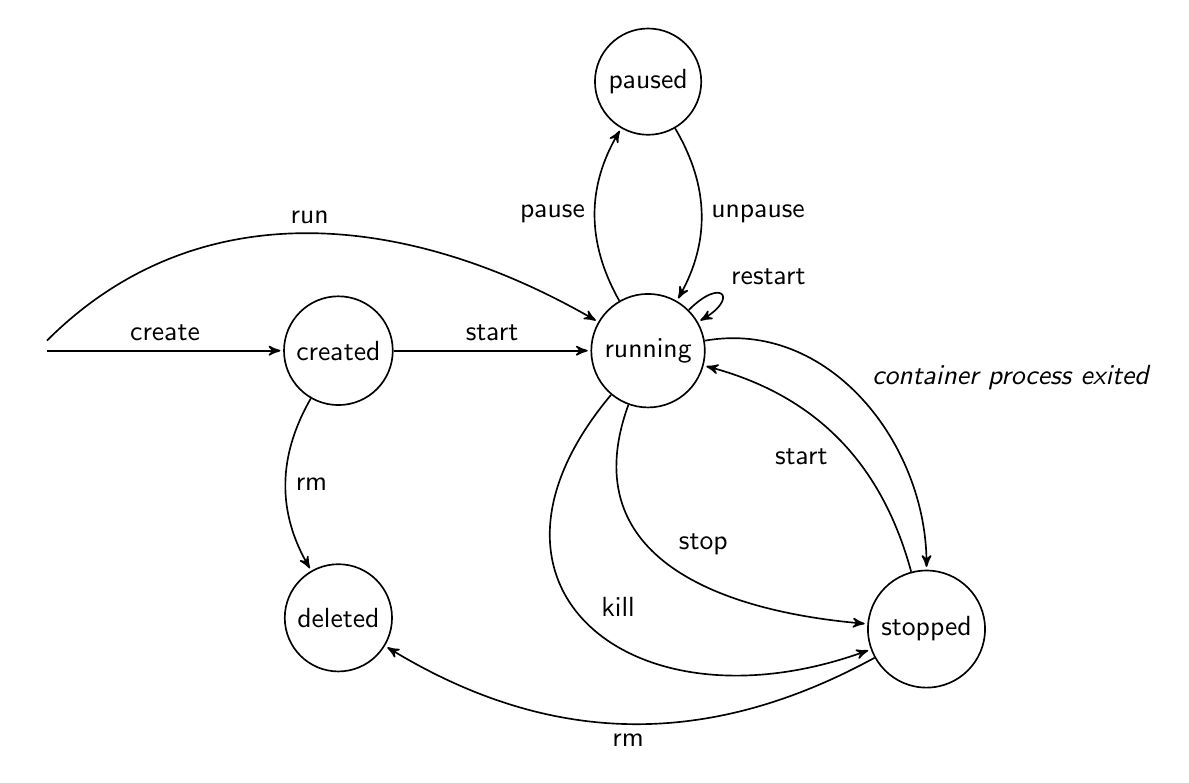
\begin{tikzpicture}[scale=0.8,->,>=stealth',shorten >=1pt,auto,node distance=5cm, semithick]
        \sffamily\fontsize{10}{10}\selectfont
        \node (cr){};
        \node (run){};
        \node[state] (A)     [right =3cm of cr]         {created};
        \node[state]         (B) [right =2.5cm of A] {running};
        \node[state]         (C) [below right of=B] {stopped};
        \node[state]         (D) [above =2cm of B] {paused};
        \node[state]         (E) [below =2cm of A] {deleted};

        \path (cr) edge [] node {create} (A)
            (run) edge [out=45,in=150]                     node {run} (B)
              (A) edge []                              node {start} (B)
                  edge [bend right]                    node {rm}    (E)
              (B) edge [out=230, in=200, distance=4cm] node {kill}  (C)
                  edge [out=250,in=175, distance=2.5cm]node {stop}  (C)
                  edge [bend left]                     node {pause}  (D)
                  edge [in=30, out=45, loop]           node {restart}  (D)
                  edge [out=10, in=90, distance=2cm]   node {\textit{container process exited}}  (C)
              (C) edge [bend right]                    node {start}  (B)
                  edge [bend left]                     node {rm}  (E)
              (D) edge [bend left]                     node {unpause} (B)
              ;
      \end{tikzpicture}
      \caption*{Simplified version. Commands should be understood prefixed with \texttt{docker}. \newline \scriptsize Based on https://docs.docker.com/engine/reference/api/docker\_remote\_api/\#docker-events }
      \caption[Docker Container Life Cycle]{Docker Container Life Cycle \cite{Docker2016Docker}}
      \label{fig:docker_container_lifecycle}
    \end{figure}

\AnhChapter{Architecture and design}

  \begin{figure}[htbp]
    \centering
    \includegraphics[width=0.65\textwidth]{content/images/class_diagram_organization-crop.pdf}
    \caption{UML Class Diagram for the Organization Service}
  \label{fig:uml_class_diagram_organization}
  \end{figure}

 \clearpage
\AnhChapter{Implementation}
  \AnhSection{Workflow image}

    \begin{listing}[!h]
      \inputminted[fontsize=\footnotesize,linenos=true,numberblanklines=true,showspaces=false,breaklines=true,baselinestretch=1]{json}{./content/snippets/process_definition.json}
      \caption{Exported process definition in JSON format}
    \label{lst:exported_process_definition_in_json_format}
    \end{listing}

    \begin{listing}[!h]
      \inputminted[fontsize=\footnotesize,linenos=true,numberblanklines=true,showspaces=false,breaklines=true,baselinestretch=1]{json}{./content/snippets/wf_image/input.schema.json}
      \caption*{ \mintinline{json}| {"this":"is a test"} | would be considered valid input data with the depicted schema }
      \caption{JSON schema used for input validation}
    \label{lst:input_schema_in_json_format}
    \end{listing}

    \begin{listing}[!h]
      \inputminted[fontsize=\footnotesize,linenos=true,numberblanklines=true,showspaces=false,breaklines=true,baselinestretch=1]{Dockerfile}{../code/wf_base/Dockerfile}
      \caption{Dockerfile for workflow base image}
    \label{lst:dockerfile_for_workflow_base_image}
    \end{listing}

    \begin{listing}[!h]
      \inputminted[lastline=39,fontsize=\footnotesize,linenos=true,numberblanklines=true,showspaces=false,breaklines=true,baselinestretch=1]{ruby}{../code/wf_base/activity_instance.rb}
      \caption{ActivityInstance class in workflow image (1/2)}
    \label{lst:wf_image_activity_instance}
    \end{listing}

    \begin{listing}[!h]
      \inputminted[firstline=40,fontsize=\footnotesize,linenos=true,numberblanklines=true,showspaces=false,breaklines=true,baselinestretch=1]{ruby}{../code/wf_base/activity_instance.rb}
      \caption{ActivityInstance class in workflow image (2/2)}
    \label{lst:wf_image_activity_instance_2}
    \end{listing}

    \begin{listing}[!h]
      \inputminted[fontsize=\footnotesize,linenos=true,numberblanklines=true,showspaces=false,breaklines=true,baselinestretch=1]{ruby}{../code/wf_base/file_helper.rb}
      \caption{FileHelper helper class in workflow image}
    \label{lst:wf_image_file_helper}
    \end{listing}
    ** overflow

    \begin{listing}[!h]
      \inputminted[fontsize=\footnotesize,linenos=true,numberblanklines=true,showspaces=false,breaklines=true,baselinestretch=1]{ruby}{../code/wf_base/process_definition.rb}
      \caption{ProcessDefinition class in workflow image}
    \label{lst:wf_image_process_definition}
    \end{listing}

    \begin{listing}[!h]
      \inputminted[lastline=45,fontsize=\footnotesize,linenos=true,numberblanklines=true,showspaces=false,breaklines=true,baselinestretch=1]{ruby}{../code/wf_base/process_instance.rb}
      \caption{ProcessInstance class in workflow image (1/2)}
    \label{lst:wf_image_process_instance}
    \end{listing}

    \begin{listing}[!h]
      \inputminted[firstline=46,fontsize=\footnotesize,linenos=true,numberblanklines=true,showspaces=false,breaklines=true,baselinestretch=1]{ruby}{../code/wf_base/process_instance.rb}
      \caption{ProcessInstance class in workflow image (2/2)}
    \label{lst:wf_image_process_instance_2}
    \end{listing}

    \begin{listing}[!h]
      \inputminted[fontsize=\footnotesize,linenos=true,numberblanklines=true,showspaces=false,breaklines=true,baselinestretch=1]{ruby}{../code/wf_base/run.rb}
      \caption{Workflow image run script}
    \label{lst:wf_image_run}
    \end{listing}

  \clearpage
  \AnhSection{Activity image}

    \begin{listing}[!h]
      \inputminted[fontsize=\footnotesize,linenos=true,numberblanklines=true,showspaces=false,breaklines=true,baselinestretch=1]{Dockerfile}{../code/ac_base/Dockerfile}
      \caption{Dockerfile for activity base image}
    \label{lst:dockerfile_for_activity_base_image}
    \end{listing}

    \begin{listing}[!h]
      \inputminted[firstline=8,lastline=58,fontsize=\footnotesize,linenos=true,numberblanklines=true,showspaces=false,breaklines=true,baselinestretch=1]{ruby}{../code/ac_base/run.rb}
      \caption{Activity instance class (1/2)}
    \label{lst:activity_instance_class}
    \end{listing}

    \begin{listing}[!h]
      \inputminted[firstline=59,fontsize=\footnotesize,linenos=true,numberblanklines=true,showspaces=false,breaklines=true,baselinestretch=1]{ruby}{../code/ac_base/run.rb}
      \caption{Activity instance class (2/2)}
    \label{lst:activity_instance_class_2}
    \end{listing}

    \begin{listing}[!h]
      \inputminted[fontsize=\footnotesize,linenos=true,numberblanklines=true,showspaces=false,breaklines=true,baselinestretch=1]{ruby}{../code/ac_base/container_invocation.rb}
      \caption{ContainerInvocation helper class}
    \label{lst:container_invocation_helper_class}
    \end{listing}

    \begin{listing}[!h]
      \inputminted[lastline=42,fontsize=\footnotesize,linenos=true,numberblanklines=true,showspaces=false,breaklines=true,baselinestretch=1]{ruby}{../code/ac_base/subworkflow_invocation.rb}
      \caption{SubworkflowInvocation helper class (1/2)}
    \label{lst:subworkflow_invocation_helper_class}
    \end{listing}

    \begin{listing}[!h]
      \inputminted[firstline=43,fontsize=\footnotesize,linenos=true,numberblanklines=true,showspaces=false,breaklines=true,baselinestretch=1]{ruby}{../code/ac_base/subworkflow_invocation.rb}
      \caption{SubworkflowInvocation helper class (2/2)}
    \label{lst:subworkflow_invocation_helper_class_2}
    \end{listing}

    \begin{listing}[!h]
      \inputminted[lastline=53,fontsize=\footnotesize,linenos=true,numberblanklines=true,showspaces=false,breaklines=true,baselinestretch=1]{ruby}{../code/ac_base/worklist_client.rb}
      \caption{WorklistClient class (1/2)}
    \label{lst:worklist_client_class}
    \end{listing}

    \begin{listing}[!h]
      \inputminted[firstline=54,fontsize=\footnotesize,linenos=true,numberblanklines=true,showspaces=false,breaklines=true,baselinestretch=1]{ruby}{../code/ac_base/worklist_client.rb}
      \caption{WorklistClient class (2/2)}
    \label{lst:worklist_client_class_2}
    \end{listing}

    \begin{listing}[!h]
      \inputminted[fontsize=\footnotesize,linenos=true,numberblanklines=true,showspaces=false,breaklines=true,baselinestretch=1]{json}{./content/snippets/ac_image/activity.info.json}
      \caption{Activity information for the inclusion in the activity image}
    \label{lst:activity_info_json}
    \end{listing}


    ** get lines right everywhere

  \clearpage
  \AnhSection{Workflow definition service}

    \begin{listing}[!h]
      \inputminted[fontsize=\footnotesize,linenos=true,numberblanklines=true,showspaces=false,breaklines=true,baselinestretch=1]{ruby}{../code/definition/definition.rb}
      \caption{Definition service run script}
    \label{lst:definition_run}
    \end{listing}

    \begin{listing}[!h]
      \inputminted[fontsize=\footnotesize,linenos=true,numberblanklines=true,showspaces=false,breaklines=true,baselinestretch=1]{ruby}{../code/definition/serializers/process_definition_image_serializer.rb}
      \caption{ProcessDefinitionImageSerializer class}
    \label{lst:process_definition_image_serializer}
    \end{listing}

    \begin{listing}[!h]
      \inputminted[fontsize=\footnotesize,linenos=true,numberblanklines=true,showspaces=false,breaklines=true,baselinestretch=1]{ruby}{../code/definition/serializers/workflow_full_serializer.rb}
      \caption{WorkflowFullSerializer class}
    \label{lst:workflow_full_serializer}
    \end{listing}

    \begin{listing}[!h]
      \inputminted[fontsize=\footnotesize,linenos=true,numberblanklines=true,showspaces=false,breaklines=true,baselinestretch=1]{ruby}{../code/definition/models/activity.rb}
      \caption{Activity class}
    \label{lst:activity}
    \end{listing}

    \begin{listing}[!h]
      \inputminted[fontsize=\footnotesize,linenos=true,numberblanklines=true,showspaces=false,breaklines=true,baselinestretch=1]{ruby}{../code/definition/models/control_flow.rb}
      \caption{ControlFlow class}
    \label{lst:control_flow}
    \end{listing}

    \begin{listing}[!h]
      \inputminted[fontsize=\footnotesize,linenos=true,numberblanklines=true,showspaces=false,breaklines=true,baselinestretch=1]{ruby}{../code/definition/models/process_definition.rb}
      \caption{ProcessDefinition class}
    \label{lst:process_definition}
    \end{listing}

    \begin{listing}[!h]
      \inputminted[fontsize=\footnotesize,linenos=true,numberblanklines=true,showspaces=false,breaklines=true,baselinestretch=1]{ruby}{../code/definition/models/workflow.rb}
      \caption{Workflow class}
    \label{lst:workflow}
    \end{listing}

    \begin{listing}[!h]
      \inputminted[fontsize=\footnotesize,linenos=true,numberblanklines=true,showspaces=false,breaklines=true,baselinestretch=1]{ruby}{../code/definition/lib/image_builder.rb}
      \caption{ImageBuilder class}
    \label{lst:image_builder}
    \end{listing}

    \begin{listing}[!h]
      \inputminted[fontsize=\footnotesize,linenos=true,numberblanklines=true,showspaces=false,breaklines=true,baselinestretch=1]{ruby}{../code/definition/lib/image_manager.rb}
      \caption{ImageManager class}
    \label{lst:image_manager}
    \end{listing}

    \begin{listing}[!h]
      \inputminted[fontsize=\footnotesize,linenos=true,numberblanklines=true,showspaces=false,breaklines=true,baselinestretch=1]{ruby}{../code/definition/consumers/activity_consumer.rb}
      \caption{ActivityConsumer class}
    \label{lst:activity_consumer}
    \end{listing}

    \begin{listing}[!h]
      \inputminted[fontsize=\footnotesize,linenos=true,numberblanklines=true,showspaces=false,breaklines=true,baselinestretch=1]{ruby}{../code/definition/consumers/control_flow_consumer.rb}
      \caption{ControlFlowConsumer class}
    \label{lst:control_flow_consumer}
    \end{listing}

    \begin{listing}[!h]
      \inputminted[fontsize=\footnotesize,linenos=true,numberblanklines=true,showspaces=false,breaklines=true,baselinestretch=1]{ruby}{../code/definition/consumers/docker_consumer.rb}
      \caption{DockerConsumer class}
    \label{lst:docker_consumer}
    \end{listing}

    \begin{listing}[!h]
      \inputminted[fontsize=\footnotesize,linenos=true,numberblanklines=true,showspaces=false,breaklines=true,baselinestretch=1]{ruby}{../code/definition/consumers/process_definition_consumer.rb}
      \caption{ProcessDefinitionConsumer class}
    \label{lst:process_definition_consumer}
    \end{listing}

    \begin{listing}[!h]
      \inputminted[fontsize=\footnotesize,linenos=true,numberblanklines=true,showspaces=false,breaklines=true,baselinestretch=1]{ruby}{../code/definition/consumers/workflow_consumer.rb}
      \caption{WorkflowConsumer class}
    \label{lst:workflow_consumer}
    \end{listing}

  \clearpage
  \AnhSection{Developer gateway}

    \begin{listing}[!h]
      \inputminted[fontsize=\footnotesize,linenos=true,numberblanklines=true,showspaces=false,breaklines=true,baselinestretch=1]{ruby}{../code/developer_gateway/app/controllers/application_controller.rb}
      \caption{ApplicationController class in developer gateway}
    \label{lst:application_controller_class_in_developer_gateway}
    \end{listing}

    \begin{listing}[!h]
      \inputminted[fontsize=\footnotesize,linenos=true,numberblanklines=true,showspaces=false,breaklines=true,baselinestretch=1]{ruby}{../code/developer_gateway/app/controllers/workflows_controller.rb}
      \caption{WorkflowsController class in developer gateway}
    \label{lst:workflows_controller_class_in_developer_gateway}
    \end{listing}

  \clearpage
  \AnhSection{Workflow engine service}

    \begin{listing}[!h]
      \inputminted[fontsize=\footnotesize,linenos=true,numberblanklines=true,showspaces=false,breaklines=true,baselinestretch=1]{ruby}{../code/engine/wf_engine.rb}
      \caption{WorkflowEngine class in workflow engine service}
    \label{lst:wf_engine_class_in_workflow_engine_service}
    \end{listing}

    \begin{listing}[!h]
      \inputminted[fontsize=\footnotesize,linenos=true,numberblanklines=true,showspaces=false,breaklines=true,baselinestretch=1]{ruby}{../code/engine/consumers/workflow_consumer.rb}
      \caption{WorkflowConsumer class in workflow engine service}
    \label{lst:workflow_consumer_class_in_workflow_engine_service}
    \end{listing}

    \begin{listing}[!h]
      \inputminted[fontsize=\footnotesize,linenos=true,numberblanklines=true,showspaces=false,breaklines=true,baselinestretch=1]{ruby}{../code/engine/consumers/workflow_instance_consumer.rb}
      \caption{WorkflowInstanceConsumer class in workflow engine service}
    \label{lst:workflow_instance_consumer_class_in_workflow_engine_service}
    \end{listing}

    \begin{listing}[!h]
      \inputminted[fontsize=\footnotesize,linenos=true,numberblanklines=true,showspaces=false,breaklines=true,baselinestretch=1]{ruby}{../code/engine/lib/workflow_instance.rb}
      \caption{WorkflowInstance class in workflow engine service}
    \label{lst:workflow_instance_class_in_workflow_engine_service}
    \end{listing}

    \begin{listing}[!h]
      \inputminted[fontsize=\footnotesize,linenos=true,numberblanklines=true,showspaces=false,breaklines=true,baselinestretch=1]{ruby}{../code/engine/lib/docker_helper.rb}
      \caption{DockerHelper class in workflow engine service}
    \label{lst:docker_helper_class_in_workflow_engine_service}
    \end{listing}

  \clearpage
  \AnhSection{Event converter service}
    \begin{listing}[!h]
      \inputminted[fontsize=\footnotesize,linenos=true,numberblanklines=true,showspaces=false,breaklines=true,baselinestretch=1]{ruby}{../code/event_converter/event_converter.rb}
      \caption{Conversion of Docker events to \ac{MOM} messages}
    \label{lst:conversion_of_docker_events_to_mom_messages}
    \end{listing}

  \clearpage
  \AnhSection{Infrastructure management service}
    \begin{listing}[!h]
      \inputminted[fontsize=\footnotesize,linenos=true,numberblanklines=true,showspaces=false,breaklines=true,baselinestretch=1]{ruby}{../code/infrastructure/consumers/server_consumer.rb}
      \caption{ServerConsumer class in infrastructure managment service}
    \label{lst:server_consumer_in_infrastructure_managment_service}
    \end{listing}

    \begin{listing}[!h]
      \inputminted[fontsize=\footnotesize,linenos=true,numberblanklines=true,showspaces=false,breaklines=true,baselinestretch=1]{ruby}{../code/infrastructure/lib/docker_helper.rb}
      \caption{DockerHelper class in infrastructure managment service}
    \label{lst:docker_helper_in_infrastructure_managment_service}
    \end{listing}

    \begin{listing}[!h]
      \inputminted[fontsize=\footnotesize,linenos=true,numberblanklines=true,showspaces=false,breaklines=true,baselinestretch=1]{ruby}{../code/infrastructure/lib/environment_manager.rb}
      \caption{EnvironmentManager class in infrastructure managment service}
    \label{lst:environment_manager_in_infrastructure_managment_service}
    \end{listing}

  \clearpage
  \AnhSection{Organization management service}
    \begin{listing}[!h]
      \inputminted[fontsize=\footnotesize,linenos=true,numberblanklines=true,showspaces=false,breaklines=true,baselinestretch=1]{ruby}{../code/organization/consumers/role_consumer.rb}
      \caption{RoleConsumer class in organization managment service}
    \label{lst:role_consumer_in_organization_managment_service}
    \end{listing}

    \begin{listing}[!h]
      \inputminted[fontsize=\footnotesize,linenos=true,numberblanklines=true,showspaces=false,breaklines=true,baselinestretch=1]{ruby}{../code/organization/models/role.rb}
      \caption{Role class in organization managment service}
    \label{lst:role_in_organization_managment_service}
    \end{listing}

  \clearpage
  \AnhSection{Provisioning service}
    \begin{listing}[!h]
      \inputminted[fontsize=\footnotesize,linenos=true,numberblanklines=true,showspaces=false,breaklines=true,baselinestretch=1]{ruby}{../code/provisioner/provisioner.rb}
      \caption{Provisioning service}
    \label{lst:provisioning_service}
    \end{listing}

  \clearpage
  \AnhSection{User gateway}

    \begin{listing}[!h]
      \inputminted[fontsize=\footnotesize,linenos=true,numberblanklines=true,showspaces=false,breaklines=true,baselinestretch=1]{ruby}{../code/user_gateway/app/controllers/worklists_controller.rb}
      \caption{WorklistsController class in user gateway}
    \label{lst:worklists_controller_class_in_user_gateway}
    \end{listing}

    \begin{listing}[!h]
      \inputminted[fontsize=\footnotesize,linenos=true,numberblanklines=true,showspaces=false,breaklines=true,baselinestretch=1]{ruby}{../code/user_gateway/app/controllers/worklist_items_controller.rb}
      \caption{WorklistItemsController class in user gateway}
    \label{lst:worklist_items_controller_class_in_user_gateway}
    \end{listing}

  \clearpage
  \AnhSection{Worklist handler service}
    \begin{listing}[!h]
      \inputminted[fontsize=\footnotesize,linenos=true,numberblanklines=true,showspaces=false,breaklines=true,baselinestretch=1]{ruby}{../code/worklist/consumers/user_consumer.rb}
      \caption{UserConsumer class in worklist managment service}
    \label{lst:user_consumer_in_worklist_managment_service}
    \end{listing}

    \begin{listing}[!h]
      \inputminted[fontsize=\footnotesize,linenos=true,numberblanklines=true,showspaces=false,breaklines=true,baselinestretch=1]{ruby}{../code/worklist/consumers/worklist_consumer.rb}
      \caption{WorklistConsumer class in worklist managment service}
    \label{lst:worklist_consumer_in_worklist_managment_service}
    \end{listing}

    \begin{listing}[!h]
      \inputminted[fontsize=\footnotesize,linenos=true,numberblanklines=true,showspaces=false,breaklines=true,baselinestretch=1]{ruby}{../code/worklist/models/worklist_item.rb}
      \caption{WorklistItem class in worklist managment service}
    \label{lst:worklist_item_in_organization_managment_service}
    \end{listing}

\clearpage
\AnhChapter{Deployment}

  \begin{figure}[htbp]
    \centering
    \includegraphics[width=0.95\textwidth]{content/images/Architecture-crop.pdf}
    \caption*{\scriptsize Note: the depicted distribution of containers to nodes is just exemplarily. Most of them could run on any node in the swarm. The only mandatory assignments are the swarm agents, of which each node needs one, and the provisioners, of which each node that is intended to execute workflows on needs one. \\ Also, the databases and their respective data volumes were omitted for the sake of clarity. ** LAN WAN**}
    \caption{UML deployment diagram of the architecture}
    \label{fig:deployment_diagram_of_the_architecture}
  \end{figure}

  \begin{listing}[!htbp]
    \inputminted[lastline=47,fontsize=\footnotesize,linenos=true,numberblanklines=true,showspaces=false,breaklines=true,baselinestretch=1]{bash}{../code/_setup/setup_1_environment.sh}
    \caption{Setup of the machines for the exemplary deployment (1/2) }
  \label{lst:setup_exemplary_deployment_1}
  \end{listing}

  \begin{listing}[!htbp]
    \inputminted[firstline=48,fontsize=\footnotesize,linenos=true,numberblanklines=true,showspaces=false,breaklines=true,baselinestretch=1]{bash}{../code/_setup/setup_1_environment.sh}
    \caption{Setup of the machines for the exemplary deployment (2/2) }
  \label{lst:setup_exemplary_deployment_1_2}
  \end{listing}

  \begin{listing}[!htbp]
    \inputminted[firstline=48,fontsize=\footnotesize,linenos=true,numberblanklines=true,showspaces=false,breaklines=true,baselinestretch=1]{bash}{../code/_setup/setup_2_dev_services.sh}
    \caption{Setup of the services for the exemplary deployment }
  \label{lst:setup_exemplary_deployment_2}
  \end{listing}

  \begin{listing}[!htbp]
    \inputminted[lastline=50,fontsize=\footnotesize,linenos=true,numberblanklines=true,showspaces=false,breaklines=true,baselinestretch=1]{yaml}{../code/wfms.yml}
    \caption{The whole Docker Compose file of the \ac{WfMS} (1/5)}
  \label{lst:the_whole_docker_compose_file_1}
  \end{listing}

  \begin{listing}[!htbp]
    \inputminted[firstline=51,lastline=98,fontsize=\footnotesize,linenos=true,numberblanklines=true,showspaces=false,breaklines=true,baselinestretch=1]{yaml}{../code/wfms.yml}
    \caption{The whole Docker Compose file of the \ac{WfMS} (2/5)}
  \label{lst:the_whole_docker_compose_file_2}
  \end{listing}

  \begin{listing}[!htbp]
    \inputminted[firstline=99,lastline=145,fontsize=\footnotesize,linenos=true,numberblanklines=true,showspaces=false,breaklines=true,baselinestretch=1]{yaml}{../code/wfms.yml}
    \caption{The whole Docker Compose file of the \ac{WfMS} (3/5)}
  \label{lst:the_whole_docker_compose_file_3}
  \end{listing}

  \begin{listing}[!htbp]
    \inputminted[firstline=146,lastline=197,fontsize=\footnotesize,linenos=true,numberblanklines=true,showspaces=false,breaklines=true,baselinestretch=1]{yaml}{../code/wfms.yml}
    \caption{The whole Docker Compose file of the \ac{WfMS} (4/5)}
  \label{lst:the_whole_docker_compose_file_4}
  \end{listing}

  \begin{listing}[!htbp]
    \inputminted[firstline=198,fontsize=\footnotesize,linenos=true,numberblanklines=true,showspaces=false,breaklines=true,baselinestretch=1]{yaml}{../code/wfms.yml}
    \caption{The whole Docker Compose file of the \ac{WfMS} (5/5)}
  \label{lst:the_whole_docker_compose_file_5}
  \end{listing}

\clearpage
\AnhChapter{Case study}

  \begin{figure}[htbp]
    \centering
    \includegraphics[width=\textwidth]{./content/images/usecase/case_study_6.png}
    \caption{Dashboard of the prototype}
    \label{fig:dashboard}
  \end{figure}

  \begin{figure}[htbp]
    \centering
    \includegraphics[width=\textwidth]{./content/images/usecase/case_study_8.png}
    \caption{Roles view of the prototype}
    \label{fig:dev_role}
  \end{figure}

  \begin{figure}[htbp]
    \centering
    \includegraphics[width=\textwidth]{./content/images/usecase/case_study_9.png}
    \caption{Users view of the prototype}
    \label{fig:dev_user}
  \end{figure}

  \begin{figure}[htbp]
    \centering
    \includegraphics[width=\textwidth]{./content/images/usecase/case_study_10.png}
    \caption{Modeling a third party container workflow}
    \label{fig:tpc_wf}
  \end{figure}

  \begin{figure}[htbp]
    \centering
    \includegraphics[width=\textwidth]{./content/images/usecase/case_study_12.png}
    \caption{Created images for the third party container workflow}
    \label{fig:tpc_images}
  \end{figure}

  \begin{figure}[htbp]
    \centering
    \includegraphics[width=\textwidth]{./content/images/usecase/case_study_13.png}
    \caption{Provisioner reacts to pushed image by initiating pull}
    \label{fig:provisioner_pulls}
  \end{figure}

  \begin{figure}[htbp]
    \centering
    \includegraphics[width=\textwidth]{./content/images/usecase/case_study_10.png}
    \caption{Modeling a manual activity workflow}
    \label{fig:manual_wf}
  \end{figure}

  \begin{figure}[htbp]
    \centering
    \includegraphics[width=\textwidth]{./content/images/usecase/case_study_26.png}
    \caption{Modeling a sub-workflow workflow}
    \label{fig:subwf_wf}
  \end{figure}

  \begin{figure}[htbp]
    \centering
    \includegraphics[width=\textwidth]{./content/images/usecase/case_study_19.png}
    \caption{Worklist overview in the user gateway}
    \label{fig:wl_index}
  \end{figure}

  \begin{figure}[htbp]
    \centering
    \includegraphics[width=\textwidth]{./content/images/usecase/case_study_20.png}
    \caption{Worklist item overview of a user in the user gateway}
    \label{fig:wl_user}
  \end{figure}

  \begin{figure}[htbp]
    \centering
    \includegraphics[width=\textwidth]{./content/images/usecase/case_study_22.png}
    \caption{Manually updating worklist item in RabbitMQ admin interface}
    \label{fig:wl_update}
  \end{figure}

  \begin{figure}[htbp]
    \centering
    \includegraphics[width=\textwidth]{./content/images/usecase/case_study_25.png}
    \caption{Executed containers for the case study}
    \label{fig:exe_containers}
  \end{figure}

  \begin{listing}[!h]
    \inputminted[fontsize=\footnotesize,linenos=true,numberblanklines=true,showspaces=false,breaklines=true,baselinestretch=1]{json}{./content/snippets/example_output_2.json}
    \caption*{Annotations are not part of the original output}
    \caption{Resulting data of the workflow enactment in the case study}
  \label{lst:resulting_data_set}
  \end{listing}




  % \renewcommand\listingscaption{List.}
  % \captionsetup[listing]{labelformat=simple}


\AbschlErklaerung{2016-03-08}
\end{document}
